\documentclass[a4paper,11pt]{book}
\usepackage{listings}
\usepackage[utf8]{inputenc}
\usepackage{titlesec}
\usepackage{fancyhdr}
\usepackage[spanish,es-tabla]{babel}
\usepackage[hidelinks]{hyperref}
\usepackage{xcolor}
\usepackage{pdfpages}

% Información reutilizable
\newcommand{\asunto}{Trabajo de Fin de Grado}
\newcommand{\titulo}{RSMap, reconocimiento y representación del tráfico}
\newcommand{\tituloEng}{RSMap, traffic analysis and recognition }
\newcommand{\grado}{Grado en Ingeniería Informática}
\newcommand{\autor}{José Manuel Luque Burgos}
\newcommand{\email}{luqueburgosjm@gmail.com}
\newcommand{\tutor}{Juan Julián Merelo Guervós}
\newcommand{\escuela}{Escuela Técnica Superior de Ingenierías Informática y de Telecomunicación}
\newcommand{\universidad}{Universidad de Granada}
\newcommand{\ciudad}{Granada}
\newcommand{\vers}{Versión 0.1}

% Información archivo
\hypersetup{
	pdfauthor = {\autor\ (\email)},
	pdftitle = {\titulo},
	pdfsubject = {\asunto},
	pdfkeywords = {smart cities, tiempo real, tráfico, raspberry pi, software libre, análisis de datos, REST api},
	pdfcreator = {LaTeX con el paquete texlive},
	pdfproducer = {pdflatex}
}

% Estilo de cabeceras
\pagestyle{fancy}
\fancyhf{}
\fancyhead[LO]{\leftmark}
\fancyhead[RE]{\rightmark}
\fancyhead[RO,LE]{\textbf{\thepage}}
\setlength{\headheight}{1.5\headheight}

% Redefinición de comandos
\renewcommand{\lstlistingname}{Fragmento de código}
\renewcommand{\lstlistlistingname}{Índice de fragmentos de código}
\renewcommand{\chaptermark}[1]{\markboth{\textbf{#1}}{}}
\renewcommand{\sectionmark}[1]{\markright{\textbf{\thesection. #1}}}

% Definición de colores
\definecolor{gray97}{gray}{.97}
\definecolor{gray75}{gray}{.75}
\definecolor{gray45}{gray}{.45}
\definecolor{gray30}{gray}{.94}
\definecolor{lightgray}{rgb}{.9,.9,.9}
\definecolor{darkgray}{rgb}{.4,.4,.4}
\definecolor{purple}{rgb}{0.65, 0.12, 0.82}
\definecolor{background}{HTML}{EEEEEE}
\definecolor{delim}{RGB}{20,105,176}
\colorlet{punct}{red!60!black}
\colorlet{numb}{magenta!60!black}
\definecolor{eclipseBlue}{RGB}{42,0.0,255}
\definecolor{eclipseGreen}{RGB}{63,127,95}
\definecolor{eclipsePurple}{RGB}{127,0,85}

% Listados
\lstset{
	aboveskip=0.5cm,
	backgroundcolor=\color{gray97},
	basicstyle=\scriptsize\ttfamily,
	breaklines=true,
	commentstyle=\color{gray45},
	frame=Ltb,
	framerule=0.5pt,
	framesep=0pt,
	framexbottommargin=3pt,
	framexleftmargin=0.1cm,
	framextopmargin=3pt,
	keywordstyle=\bfseries,
	numberfirstline = false,
	numbers=left,
	numbersep=6pt,
	numberstyle=\tiny,
	rulesep=.4pt,
	rulesepcolor=\color{black},
	showstringspaces = false,
	stringstyle=\ttfamily,
	literate={á}{{\'a}}1
	         {é}{{\'e}}1
	         {í}{{\'i}}1
	         {ó}{{\'o}}1
	         {ú}{{\'u}}1
	         {ñ}{{\~n}}1
}

% Minimizar fragmentado de listados
\lstnewenvironment{listing}[1][]
	{\lstset{#1}\pagebreak[0]}{\pagebreak[0]}

% Listado definido para JavaScript
% http://tex.stackexchange.com/questions/89574/language-option-supported-in-listings/89576#89576
\lstdefinelanguage{javascript}{
	backgroundcolor=\color{background},
	basicstyle=\footnotesize,
	breaklines=true,
	captionpos=b,
	comment=[l]{//},
	commentstyle=\color{purple}\ttfamily,
	frame=lines,
	identifierstyle=\color{black},
	keywordstyle=\color{blue}\bfseries,
	morecomment=[s]{/*}{*/},
	morestring=[b]',
	morestring=[b]",
	ndkeywordstyle=\color{darkgray}\bfseries,
	numbers=left,
	numbersep=8pt,
	numberstyle=\scriptsize,
	sensitive=false,
	showstringspaces=false,
	stepnumber=1,
	stringstyle=\color{red}\ttfamily,
	keywords={
		break,
		case,
		catch,
		catch,
		do,
		else,
		false,
		function,
		if,
		in,
		new,
		null,
		return,
		switch,
		true,
		typeof,
		var,
		while},
	ndkeywords={
		boolean,
		class,
		export,
		implements,
		import,
		this,
		throw}
}

% Listado definido para JSON
% http://tex.stackexchange.com/questions/83085/how-to-improve-listings-display-of-json-files/83100#83100
\lstdefinelanguage{json}{
	backgroundcolor=\color{background},
	basicstyle=\footnotesize,
	breaklines=true,
	captionpos=b,
	frame=lines,
	numbers=left,
	numbersep=8pt,
	numberstyle=\scriptsize,
	showstringspaces=false,
	stepnumber=1,
	literate=
		*{:}{{{\color{punct}{:}}}}{1}
		{,}{{{\color{punct}{,}}}}{1}
	    {\{}{{{\color{delim}{\{}}}}{1}
	    {\}}{{{\color{delim}{\}}}}}{1}
	    {[}{{{\color{delim}{[}}}}{1}
	    {]}{{{\color{delim}{]}}}}{1}
	    {ñ}{{\~{n}}}{1}
}

% Listado java
%
\lstdefinelanguage{python}{
	backgroundcolor=\color{background},
	basicstyle=\footnotesize,
	breaklines=true,
	captionpos=b,
	comment=[l]{#},
	commentstyle=\color{purple}\ttfamily,
	frame=lines,
	identifierstyle=\color{black},
	keywordstyle=\color{blue}\bfseries,
	morecomment=[s]{/*}{*/},
	morestring=[b]',
	morestring=[b]",
	ndkeywordstyle=\color{darkgray}\bfseries,
	numbers=left,
	numbersep=8pt,
	numberstyle=\scriptsize,
	sensitive=false,
	showstringspaces=false,
	stepnumber=1,
	stringstyle=\color{red}\ttfamily,
	keywords={
		break,
		case,
		catch,
		catch,
		do,
		else,
		False,
		function,
		if,
		in,
		new,
		null,
		return,
		switch,
		True,
		typeof,
		var,
		while,
		public,
		static,
		void,
		with,
		main,},
	ndkeywords={
		boolean,
		class,
		export,
		String,
		implements,
		import,
		from,
		as,
		this,
		throw}
}

% Listado java
%
\lstdefinelanguage{java}{
	backgroundcolor=\color{background},
	basicstyle=\footnotesize,
	breaklines=true,
	captionpos=b,
	comment=[l]{//},
	commentstyle=\color{purple}\ttfamily,
	frame=lines,
	identifierstyle=\color{black},
	keywordstyle=\color{blue}\bfseries,
	morecomment=[s]{/*}{*/},
	morestring=[b]',
	morestring=[b]",
	ndkeywordstyle=\color{darkgray}\bfseries,
	numbers=left,
	numbersep=8pt,
	numberstyle=\scriptsize,
	sensitive=false,
	showstringspaces=false,
	stepnumber=1,
	stringstyle=\color{red}\ttfamily,
	keywords={
		break,
		case,
		catch,
		catch,
		do,
		else,
		false,
		function,
		if,
		in,
		new,
		null,
		return,
		switch,
		true,
		typeof,
		var,
		while,
		public,
		static,
		void,
		main,},
	ndkeywords={
		boolean,
		class,
		export,
		String,
		implements,
		import,
		this,
		throw}
}

% Listado bash
%
\lstdefinelanguage{bash}{
	backgroundcolor=\color{background},
	basicstyle=\footnotesize,
	breaklines=true,
	captionpos=b,
	comment=[l]{//},
	commentstyle=\color{purple}\ttfamily,
	frame=lines,
	identifierstyle=\color{black},
	keywordstyle=\color{blue}\bfseries,
	morecomment=[s]{/*}{*/},
	morestring=[b]',
	morestring=[b]",
	ndkeywordstyle=\color{darkgray}\bfseries,
	numbers=left,
	numbersep=8pt,
	numberstyle=\scriptsize,
	sensitive=false,
	showstringspaces=false,
	stepnumber=1,
	stringstyle=\color{red}\ttfamily,
	keywords={
		sudo,
		dd,
		lsblk,
		lsusb,
		$,
		apt-get,
		aplay,
		},
	ndkeywords={
		boolean,
		class,
		export,
		String,
		implements,
		import,
		this,
		throw}
}

% Listado CQL
%
\lstdefinelanguage{cql}{
	backgroundcolor=\color{background},
	basicstyle=\footnotesize,
	breaklines=true,
	captionpos=b,
	comment=[l]{//},
	commentstyle=\color{purple}\ttfamily,
	frame=lines,
	identifierstyle=\color{black},
	keywordstyle=\color{blue}\bfseries,
	morecomment=[s]{/*}{*/},
	morestring=[b]',
	morestring=[b]",
	ndkeywordstyle=\color{darkgray}\bfseries,
	numbers=left,
	numbersep=8pt,
	numberstyle=\scriptsize,
	sensitive=false,
	showstringspaces=false,
	stepnumber=1,
	stringstyle=\color{red}\ttfamily,
	keywords={
		SELECT,
		FROM,
		WHERE,
		AND,
		ORDER BY,
		ASC,
		AS,
		},
	ndkeywords={
		boolean,
		class,
		export,
		String,
		implements,
		import,
		this,
		throw}
}


% Para que las páginas en blanco no tengan cabecera
\makeatletter
\def\clearpage{%
  \ifvmode
    \ifnum \@dbltopnum =\m@ne
      \ifdim \pagetotal <\topskip
        \hbox{}
      \fi
    \fi
  \fi
  \newpage
  \thispagestyle{empty}
  \write\m@ne{}
  \vbox{}
  \penalty -\@Mi
}
\makeatother

\begin{document}
\begin{titlepage}

\newlength{\centeroffset}
\setlength{\centeroffset}{-0.5\oddsidemargin}
\addtolength{\centeroffset}{0.5\evensidemargin}

\noindent\hspace*{\centeroffset}\begin{minipage}{\textwidth}

\centering

\includegraphics[width=0.9\textwidth]{../images/logo_ugr.png}\\[1.4cm]

\textsc{\Large\asunto\\[0.2cm]}
\textsc{\grado}\\[1cm]

{\Huge\bfseries \titulo\\}
\noindent\rule[-1ex]{\textwidth}{3pt}\\[3.5ex]
\end{minipage}

\vspace{2cm}
\noindent\hspace*{\centeroffset}\begin{minipage}{\textwidth}
\centering

\textbf{Autor}\\ {\autor}\\[2.5ex]
\textbf{Tutor}\\ {\tutor}\\[2cm]

\includegraphics[width=0.3\textwidth]{../images/logo_etsiit.png}\\[0.1cm]
\textsc{\escuela}\\
\textsc{---}\\
\ciudad, \today\\

\includegraphics[width=0.3\textwidth]{../images/CC-SA-logo.png}
\end{minipage}
\end{titlepage}
\frontmatter
\begin{center}
{\LARGE\bfseries\titulo}\\
\end{center}
\begin{center}
\autor\
\end{center}

\section*{Resumen}

\bigskip
\noindent{\textbf{Palabras clave}: \textit{smart cities}, \textit{tiempo real}, \textit{tráfico}, \textit{sensores}, \textit{análisis de datos}, \textit{software libre}\\

RSMap es un conjunto de tecnologías que trabajan en conjunto con el propósito de ofrecer información en tiempo real del estado del tráfico.

\bigskip
La información es recolectada por sensores situados cerca de cualquier ruta por la que pasen vehículos.

Éstos dispositivos filtran mediante micrófonos el sonido ambiente de la localización en la que se encuentran y remiten la información a los elementos que conforman la parte visual y de almacenamiento de RSMap.

\bigskip

En RSMap los dispositivos recolectores envían las señales de detección de vehículos a una plataforma web mediante una API Rest. Ésta web representará las señales enviadas sobre un mapa en tiempo real permitiendo a un usuario saber en qué puntos existe tráfico. La información almacenada aquí tiene caracter temporal pues, una vez representada sobre el mapa ya no es útil pero dado que se han invertido una serie de recursos en la recolección y procesado de dicha información, ésta es aprovechada para otros propósitos.

\bigskip
En este punto RSMap se sirve de herramientas orientadas al Big Data, guardando la información obtenida en una base de datos especialmente diseñada para almacenar millones de registros.

Además RSMap incluye otra forma de visualización, que permite consultar los datos almacenados de manera masiva a lo largo del tiempo para su análisis y estudio permitiendo así, la posibilidad de optimizar el tráfico de ciudades o carreteras, ver que rutas tienen más afluencia o hacer una estimación de el caudal de vehículos que circulará por una vía en un día.

\newpage
\begin{center}
{\LARGE\bfseries\tituloEng}\\
\end{center}
\begin{center}
\autor\
\end{center}

\section*{Extended abstract}

\bigskip
\noindent{\textbf{Key words}: \textit{smart cities}, \textit{real time}, \textit{traffic}, \textit{sensors}, \textit{data analysis}, \textit{open source}\\

The main reason to develop a system like RSMap is the innovative related technologies needed to cover a solution. Nowadays Big Data and IOT software and techniques are growing fast as well as the preoccupation for making the cities a better place to live improving several aspects like administrative, eco-friendly, and monetary subjects. The problem that RSMap tries to solve is the perfect scenario to join these topics and technologies in one solution.
Traffic is an important element which is related to the aspects mentioned above because with an optimal traffic in a city we may reduce pollution, identify noisy zones or get a better traffic flow.

\bigskip

RSMap system allows the end-user to know the actual traffic status through several devices which are capturing the noise generated  by vehicles and interpreting it as signals which are represented in two different ways.
The \textit{'obvious'} way is to show it on a map so we can see how many vehicles are running on certain street at a certain time.

The second way, much more interesting, is the possibility of watching the massive stored data along the days to perform Big Data analysis operations for example, to use it to configure predictive models.

\bigskip
The approach of the solution is acquired by 4 main elements.

The first of them are the receptors, They are lightweight computers, (Raspberry Pi in our case). Their purpose is the collector element in RSMap system, they process and send the signals obtained with a microphone to the storage/visualization points.

As middleware platform between receptors and storage RSMap uses KAA IOT which is a great open source platform that manages a lot of devices which task is to generate and simplify the way to allow the receptors to send data to the massive storage.

The third element is the massive storage, RSMap uses Apache Cassandra which is best-in-class database storage system for time series and its conditions of scalability makes it a perfect component to perform the tasks of storage being able to store hundreds of thousands registers per day.

Related to Apache Cassandra, RSMap makes use of Apache Zeppelin which is a very modern (but powerful) tool to visualize the data stored in Apache Cassandra in several ways due to the fact that we can get the data as we want through queries.

To conclude, RSMap has a typical end-point for normal users. A Web site where they can observe the traffic in real time, the receptors send signals when they 'think' that a vehicle passed in front of them.This Web site is developed in Django and Django-Rest-Framework. Django is a great web framework developed in Python to build professional web pages and Django-Rest-Framework is a module which allows the receptors to send detected signals to the web page with POST/PATCH/PUT/DELETE requests.


\bigskip
At the end, RSMap is a set of technologies and tools assembled to perform traffic detection. However, the possibilities to adapt the system to other purposes are too many thanks to the modular system structure. If we want to catch other kind of environment information we only have to adapt the receptors code and define new models to store the data but the essence of the application would be the same.

\newpage
\thispagestyle{empty}
\
\vspace{3cm}

\noindent\rule[-1ex]{\textwidth}{2pt}\\[4.5ex]

Yo, \textbf{\autor}, alumno de la titulación \textbf{\grado} de la \textbf{\escuela\ de la \universidad}, autorizo la ubicación de la siguiente copia de mi Trabajo Fin de Grado (\textit{\titulo}) en la biblioteca del centro para que pueda ser consultada por las personas que lo deseen.

\bigskip
Toda la información relacionada con el proyecto se encuentra bajo licencia \textbf{Creative Commons Attribution-ShareAlike 4.0} (\url{https://creativecommons.org/licenses/by-sa/4.0/}), por lo que se permite el uso comercial de la obra y de las posibles obras derivadas, la distribución de las cuales se debe hacer con una licencia igual a la que regula la obra original.

\vspace{4cm}

\noindent Fdo: \autor

\vspace{2cm}

\begin{flushright}
\ciudad, a \today
\end{flushright}

\newpage
\thispagestyle{empty}
\
\vspace{3cm}

\noindent\rule[-1ex]{\textwidth}{2pt}\\[4.5ex]

D. \textbf{\tutor}, profesor del \textbf{Departamento de Arquitectura y Tecnología de Computadores} de la \textbf{\universidad}.

\vspace{0.5cm}

\vspace{0.5cm}

\textbf{Informa:}

\vspace{0.5cm}

Que el presente trabajo, titulado \textit{\textbf{\titulo}}, ha sido realizado bajo su supervisión por \textbf{\autor}, y
autoriza la defensa de dicho trabajo ante el tribunal que corresponda.

\vspace{0.5cm}

Y para que conste, expide y firma el presente informe en \ciudad\ a \today.

\vspace{1cm}

\textbf{El tutor:}

\vspace{5cm}

\noindent \textbf{\tutor}

\chapter*{Agradecimientos}
\thispagestyle{empty}

\vspace{1cm}

A mis padres Manolo y Aurora, por haberme apoyado desde el primer al último día de mi paso por la Universidad y a mi hermana Ana María por ayudarme en lo que he necesitado.

\bigskip

A mi tutor Juan Julián Merelo Guervós por confiar en mí y permitirme realizar el proyecto bajo su supervisión.

\bigskip

A mis amigos porque siempre están ahí cuando los necesito.

\bigskip

A mis compañeros de Universidad por todos los buenos y no tan buenos momentos que hemos pasado juntos.

\bigskip

Y a todas las comunidades que hacen posible que el Software Libre sea un hecho, en las que se trabaja desinteresadamente por convicciónes propias y sin ánimo de lucro.


\begingroup
\let\cleardoublepage\clearpage
  \tableofcontents
  \listoffigures
  \listoftables
  \lstlistoflistings
\endgroup

\newpage
\thispagestyle{empty}
\
\mainmatter
\chapter{Motivación e Introducción}

A día de hoy, las tecnologías han llegado a un punto en el que envuelven completamente a las personas, ciudades y el mundo entero. Cada vez son más los elementos que nos encontramos a nuestro alrededor que poseen conexión a Internet mediante la cual envían información de temperatura, humedad relativa, nuestras pulsaciones o los pasos que damos y que posteriormente podemos consultar en nuestro dispositivo móvil o el ordenador. Debido a esto y a otra gran diversidad de elementos que generan y almacenan cantidades ingentes de información han nacido nuevas ramas en la computación como son el \textbf{Big Data} o \textbf{IOT}.

\bigskip
Las ciudades sin duda alguna son uno de los mejores candidatos para el desarrollo y aplicación de éste tipo de tecnologías. Todos hemos oído hablar últimamente del término \textit{ciudad inteligente} o \textit{smart city} y es que, con la proliferación de las tecnologías citadas anteriormente así como una imperiosa necesidad de gestionar los recursos energéticos, económicos, medioambientales y administrativos de manera más eficiente han hecho necesaria la cohesión entre la tecnología y las propias ciudades.

\bigskip
Partiendo de esta base existen muchos campos en los que trabajar para hacer una ciudad mejor. Uno de los más relevantes puede ser el tráfico por el impacto que tiene y a los diversos factores que afecta.

\bigskip
Bajo estas premisas se aborda el problema de identificar el tráfico que fluye por una ciudad mediante el ruido que éste genera y poder almacenarlo con las tecnologías adecuadas para su análisis y visualización que permitirán conocer su estado, crear sistemas reguladores del mismo en base a los datos obtenidos así como poder comprobar los niveles de ruido generados en ciertas zonas.

\newpage

RSMap es capaz de detectar el tráfico que fluye por uno (o varios) puntos en los que se encuentran dispositivos  \textbf{Raspberry Pi} analizando el ruido ambiente. Una vez identificados se envían mediante una \textbf{API REST} construida con \textbf{Django Rest Framework} y se  muestran en un mapa web.La web basada en \textbf{Django} hace uso de \textbf{Ajax} para una cómoda navegación sin necesidad de refrescar la página manualmente.

El mapa es proporcionado por la API de \textbf{Google Maps}.

Por otra parte tenemos \textbf{Kaa} que es una plataforma para administrar un gran número de dispositivos. Ésta plataforma genera un \textbf{SDK} del cual se sirven los receptores para enviar de manera masiva los datos recabados al SGBD \textbf{Apache Cassandra} los cuales pueden ser consultados y descargados mediante un Notebook que proporciona \textbf{Apache Zeppelin}.

\section{Aplicaciones similares a RSMap}
\begin{itemize}
  \item Libelium (\url{http://www.libelium.com})

    Provee una red de sensores Bluetooth sobre una red ZigBee para el análisis del tráfico. Su mayor virtud e inconveniente a la vez es que es capaz de detectar el tráfico con una gran acierto pero por otra parte es necesario que los vehículos tengan Bluetooth lo cual no siempre sucede.
  \item Houston Radar (\url{http://houston-radar.com})

    Posee un detector multidireccional para identificar el tráfico pero necesita los sensores tienen una autonomía de unas dos semanas por lo que implica un mantenimiento por cada dispositivo detector.
  \item Diamond Traffic (\url{http://diamondtraffic.com/})

    Tiene una arquitectura parecida a la de un radar, ésto es un gran inconveniente pues no se pueden situar dispositivos a lo largo de una calle sin una gran alteración del entorno.
  \item Counting Cars (\url{http://www.countingcars.com})

    Posee varios tipos de detectores basados en audio y video por contrapartida el precio de cada dispositivo es desorbitado.
\end{itemize}

Un factor común que tienen todas estas plataformas es que es software propietario por lo que se desconoce el uso que se le pueden dar a los datos recabados además de tener unos costes nada asumibles si se pretende monitorizar el tráfico con muchos dispositivos.

RSMap compite ofreciendo una plataforma \textbf{Open Source}, totalmente personalizable y con costes más equilibrados.

\newpage

Mediante un análisi \textit{DAFO} podemos concluir que las \textbf{debilidades} de RSMap es que a diferencia de sus competidores, usa equipos más baratos para la recolección de datos lo cual puede suponer una pérdida de acierto a la hora de la detección del tráfico no obstante existe un margen de mejora para optimizar el algoritmo de detección de vehículos.

La \textbf{amenaza} principal es sin duda que éstas plataformas cuenta con años de trabajo lo que se traduce en una gran amplitud de clientes.

La partes que hacen atractivo a RSMap son que es totalmente libre y personalizable y que la infraestructura tiene un coste menor por tanto hablamos de claras \textbf{fortalezas} frente a sus competidores.

Por último las \textbf{oportunidades} que se proyectan son prometedoras debido al auge de las \textit{Smart Cities} luego, con un buen prototipo y técnicas de marketing se podría dar a conocer e implementar en lugares modestos e ir depurando y mejorando su funcionamiento hasta que sea capaz de funcionar óptimamente en grandes urbes.


\section{Alcance de la memoria}

El proceso técnico se encuentra detallado en el \textit{capítulo \ref{chap5}} (\textbf{Diseño}), que contiene el modelo que se pretende implementar y en el \textit{capítulo \ref{chap6}} (\textbf{Implementación}) que contiene los elementos software desarrollados.

Antes de ello se expondrán en el \textit{capítulo \ref{chap2}}  los (\textbf{Objetivos}) que se consideran necesarios para obtener una solución válida al problema; el \textit{capítulo \ref{chap3}} (\textbf{Planificación}) consta de las distintas fases a superar y en el \textit{capítulo \ref{chap4}} (\textbf{Análisis}) de los requisitos necesarios a alcanzar.

\bigskip
Por último en el \textit{capítulo \ref{chap7}} (\textbf{Pruebas}), se remiten las pruebas realizadas que corroboran el correcto funcionamiento y se concluye con el el \textit{capítulo \ref{chap8}}  (\textbf{Conclusiones y trabajos futuros}) en el cual se analiza el camino recorrido a lo largo de todas las fases anteriores así como posibles funcionalidades incorporables al sistema.

\chapter{Objetivos}

El principal objetivo del proyecto es ofrecer una aplicación web que muestre en tiempo real el estado del tráfico gracias a sensores \textit{(Raspberry Pi)} que analizan y envían la información obtenida de manera rápida y eficiente. Otro de los objetivos es ofrecer un almacenamiento robusto, escalable y replicable para manejar las grandes masas de información que se obtienen a lo largo de un día así como una herramienta para poder consultarlos y ofrecerlos de manera libre al público o entidades que deseen acceder a ellos.

\bigskip
Los objetivos se definen con más detalle a continuación:

\begin{itemize}
  \item \textbf{O1:} Desarrollar un método que permita reconocer cuando un vehículo ha pasado por la localización en la que el dispositivo recolector se encuentra.
  \item \textbf{O2:} Desarrollar una aplicación que permita a los usuarios instalar un dispositivo y aportar información del tráfico en el punto que ellos deseen.
  \item \textbf{O3:} Hacer uso de una base de datos especialmente diseñada para trabajar bajo el paradigma del Big Data.
  \item \textbf{O4:} Proveer un método fácil de consulta de los datos que el conjunto de dispositivos recolectores obtiene, para que cualquier usuario pueda consultarlos.
  \item \textbf{O5:} Dotar al sistema de una aplicación web en la que mediante un mapa, se muestren los puntos en los que están pasando vehículos.
\end{itemize}

\bigskip
Los aspectos formativos más utilizados son:
\begin{itemize}
  \item \textbf{Infraestructuras virtuales}, ya que los servicios usados son en su totalidad virtualizados así como el scripting necesario para la automatización de ciertas tareas.
  \item \textbf{Sistemas concurrentes}, debido a que al trabajar con dispositivos de un perfil medio-bajo para la recolección se hace necesario el paralelizar ciertas operaciones.
  \item \textbf{Bases de datos}, un elemento indispensable para tratar el problema que se plantea de almacenamiento de grandes cantidades de datos.
  \item \textbf{Ingeniería de servidores}, para la configuración de los distintos VPS usados.
  \item \textbf{Procesamiento digital de señales}, para un correcto entendimiento del análisis del sonido.
  \item \textbf{Desarrollo de aplicaciones para internet}, para el desarrollo de la plataforma web.
\end{itemize}

\section{Alcance de los objetivos}

El proyecto ofrecerá dos secciones en las que se podrá visualizar el estado del tráfico mediante un mapa y consultar los valores obtenidos de los dispositivos que se encuentran retransmitiendo información. Además permitirá a cualquier usuario configurar e iniciar su propio receptor para contribuir a la obtención de datos para el sistema.

\bigskip
En este caso, la aplicación hace uso del módulo desarrollado de detección de tráfico, sin embargo, el ámbito de la aplicación no se cierra exclusivamente a éste propósito ya que debido a su modularidad será posible el desarrollo y acoplamiento de distintos módulos de detección como podrían ser la temperatura, la humedad relativa o la luminosidad ó el análisis de los datos obtenidos mediante con herramientas como Apache Spark por ejemplo, quedando completamente abierto a cualquier modelo que un desarrollador quiera representar, por tanto hablamos de una herramienta completamente personalizable según las necesidades requeridas.


\section{Interdependencia de los objetivos}

Los objetivos podríamos alinearlos mentalmente a modo de una piramide inversa, el principal y sobre el que gira este proyecto es \textbf{O1} el cual va a generar la información, sin la cual el resto no tendrían sentido. Por otra parte existe una fuerte relación con \textbf{O2} ya que el mismo módulo encargado de generar la información deberá ser replicable y configurable tantas veces como se desee, de esta manera contribuimos a como se ha mencionado anteriormente, cualquier usuario pueda aportar datos al sistema.

En el siguiente escalón de la pirámide tendríamos \textbf{O3} y \textbf{O4} los cuales también están fuertemente ligados entre sí, ya que de nada nos serviría almacenar toda la información si no proveemos un método fácil para consultarla.

Por último tenemos \textbf{O5}, que al igual que los anteriores necesita consumir información, por tanto su dependencia con \textbf{O1}, es total.

\chapter{Planificación y presupuesto}

\section{Planificación}



\subsection{Metodología}

Desde el primer momento se tiene claro que para el desarrollo del proyecto se usará el método de Desarrollo Ágil basado en iteraciones, de éste modo se van obteniendo pequeñas funcionalidades del sistema, descartando las que se consideren prescindibles.

Dentro de cada iteración tenemos unas tareas que cumplir para darla por terminada como podemos observar en la \textit{Figura \ref{fig:met_agil}}, éste método incremental permite que el desarrollo se haga sobre una base sólida evitando modificaciones que afecten al funcionamiento global de la aplicación una vez éste se encuentre en un punto avanzado del desarrollo.


\begin{figure}[!ht]
  \begin{center}
    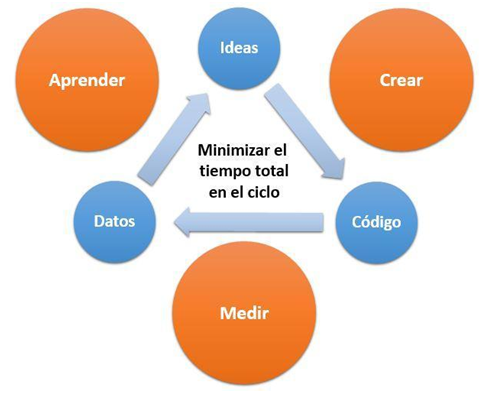
\includegraphics[scale=0.70]{../images/metodologia/agil.png}
    \caption{Metodología ágil}
    \label{fig:met_agil}
  \end{center}
\end{figure}


Por otra parte, es la manera que más natural resulta a la hora de desarrollar software pues se van completano hitos. Cada uno de ellos define una funcionalidad implementada por lo que si se desea abrir un nuevo camino \textit{(también llamados fork o roadmap)} en la aplicación tenemos varios puntos de partida evitando tener que empezar desde cero en caso de llegar a un \textit{punto muerto} en el desarrollo.

http://mprende.co/gesti%C3%B3n/agile-scrum-y-lean-startups-metodolog%C3%ADas-de-desarrollo-%C3%A1gil-de-productos

\subsection{Fases}
Tomando en consideración que la parte del proyecto referente al análisis del sonido tiene un fuerte componente teórico, se ha dedicado una sección inicial a recabar todo tipo de información relacionada con la materia para obtener una visión global y definir así un enfoque claro antes de empezar a analizar tanto las especificaciones como los requisitos. El resto de las fases son en su mayoría, comunes a cualquier proceso de elaboración de un proyecto de software.

\begin{itemize}
  \item \textbf{Fase 1:} Lecturas relacionadas con la materia del proyecto.
  \item \textbf{Fase 2:} Especificaciones y planificación.
  \item \textbf{Fase 3:} Análisis y diseño.
  \item \textbf{Fase 4:} Implementación.
  \item \textbf{Fase 5:} Pruebas.
  \item \textbf{Fase 6:} Documentación.
\end{itemize}

\newpage
\subsection{Definición y estimación de tiempo para las tareas de cada fase}

Las fases detalladas anteriormente tienen varias tareas como sub-elementos, en la siguiente lista se detalla dichos sub-elementos y la estimación aproximada para llevarla a cabo.

\begin{itemize}
   \item \textbf{Lecturas relacionadas con la materia del proyecto:}
   \begin{itemize}
    \item Como se comportan las señales.
    \item Muestreo de señales.
    \item Digitalización de señales.
    \item Identificación de patrones en señales.
    \item \underline{\textit{Duración aproximada}}: 10 días.
    \end{itemize}
\end{itemize}

\begin{itemize}
   \item \textbf{Especificaciones y planificación:}
   \begin{itemize}
    \item Objetivos.
    \item Fases.
    \item Tareas y temporización.
    \item Presupuesto.
    \item \underline{\textit{Duración aproximada:}} 4 días.
   \end{itemize}
\end{itemize}

\begin{itemize}
   \item \textbf{Análisis y diseño:}
   \begin{itemize}
    \item Análisis de requisitos.
    \item Diagramas de la aplicación.
    \item \underline{\textit{Duración aproximada:}} 20 días.
   \end{itemize}
\end{itemize}

\begin{itemize}
 \item \textbf{Implementación:}
 \begin{itemize}
  \item Selección de tecnologías.
  \item Configuración Raspberry Pi
  \item Detección de sonido
  \item Identificación de vehículos
  \item Configuración de la plataforma IOT
  \item Configuración de base de datos de almacenamiento masivo.
  \item Configuración de visualizador de los datos recolectados.
  \item Desarrollo de sistema que comunique cuando un vehículo es detectado a la plataforma web.
  \item Desarrollo de la plataforma web
  \item \underline{\textit{Duración aproximada:}} 60 días.
 \end{itemize}
\end{itemize}

Cabe destacar que al ser un proyecto en el que existen fuertes dependencias entre los objetivos, la fase de pruebas ha sido completada al mismo tiempo que la de desarrollo pues se necesitan resultados concluyentes en algunos aspectos para poder avanzar en objetivos posteriores.

\begin{itemize}
 \item \textbf{Pruebas:}
 \begin{itemize}
  \item Pruebas de detección de vehículos.
  \item Pruebas de escritura en base de datos.
  \item Pruebas de lectura de la base de datos.
  \item Pruebas de comunicación entre dispositivos y plataforma web.
  \item \underline{\textit{Duración aproximada:}} 60 días.
 \end{itemize}
\end{itemize}

La documentación al igual que las pruebas, ha ido desarrollándose al mismo tiempo que la implementación, como se puede observar en la \textit{figura 3.1}.

\begin{itemize}
 \item \textbf{Documentación:}
 \begin{itemize}
  \item Documentación del código.
  \item Documentación del proyecto.
  \item \underline{\textit{Duración aproximada:}} 60 días.
 \end{itemize}
\end{itemize}

\subsection{Diagramas de temporización}

La información acerca de la temporización queda expuesta en las siguientes figuras mediante un diagrama de fases y tareas \textit{(figura 3.1)}, un diagrama de pert \textit{(figura 3.2)} y otro de gantt \textit{(figura 3.3)} y \textit{(figura 3.4)}.

\begin{figure}[!ht]
  \begin{center}
    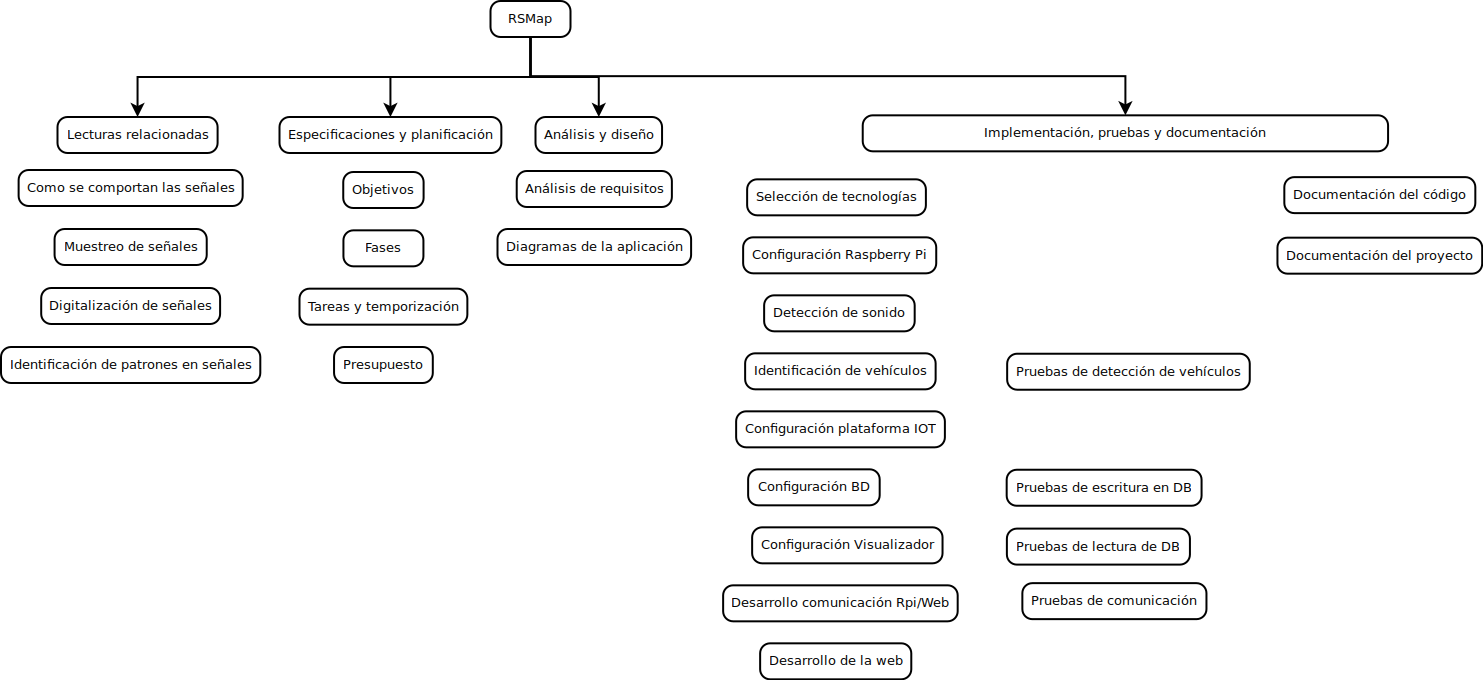
\includegraphics[scale=0.30]{../images/diag_plan/fases_tareas.png}
    \caption{Diagrama fases y tareas}
    \label{fig:fases_tareas}
  \end{center}
\end{figure}

\newpage
\begin{figure}[!ht]
  \begin{center}
    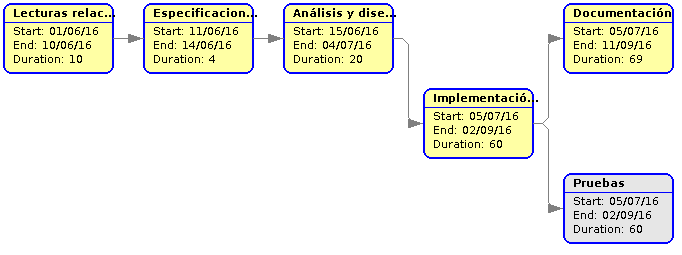
\includegraphics[width=1\textwidth]{../images/diag_plan/pert.png}
    \caption{Diagrama de pert}
    \label{fig:pert}
  \end{center}
\end{figure}

\begin{figure}[!ht]
  \begin{center}
    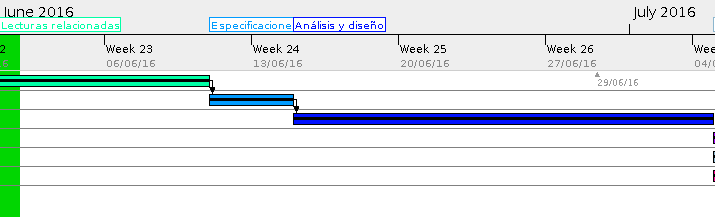
\includegraphics[width=1\textwidth]{../images/diag_plan/gantt1.png}
    \caption{Diagrama de Gantt 1}
    \label{fig:diag_gant1}
  \end{center}
\end{figure}

\begin{figure}[!ht]
  \begin{center}
    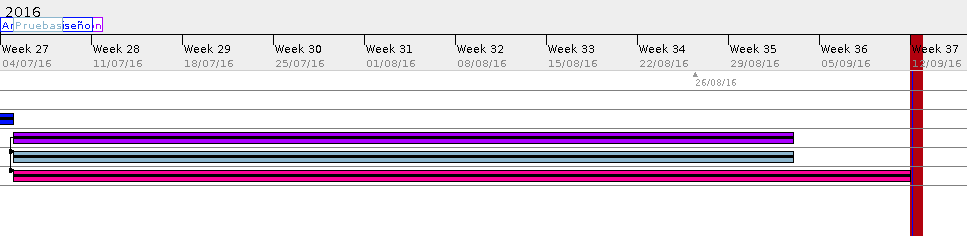
\includegraphics[width=1\textwidth]{../images/diag_plan/gantt2.png}
    \caption{Diagrama de Gantt 2}
    \label{fig:diag_gant2}
  \end{center}
\end{figure}

\newpage

\section{Presupuesto}

En el presupuesto podemos distinguir entre el software y el hardware. Por una parte el aspecto software queda totalmente cubierto de manera gratuita ya que todas las tecnologías usadas son de código abierto por tanto esto nos ahorra muchos {\textit{- por no decir todos -} los costes de este tipo.

\bigskip
El proyecto consta de los siguientes elementos software y hardware:

\bigskip
Hardware:
\begin{itemize}
	\item Raspberry Pi 2B,
	\item Tarjeta de sonido USB.
	\item Micrófono
	\item Adaptador wifi USB o cable de red RJ45.
	\item Adaptador de alimentación para la Raspberry Pi.
	\item Tarjeta SD y memoria USB.
\end{itemize}


Software:
\begin{itemize}
	\item Sistema de control de versiones para almacenar tanto la información relacionada proyecto como el código.
	\item Módulo de detección y envío de información.
	\item Plataforma IOT, que gestiona los dispositivos conectados a el sistema.
	\item Base de datos NoSQL, almacenar´a la información recolectada.
	\item Notebook que permite analizar cantidades masivas de datos almacenadas en la base de datos.
	\item REST api, la cual recibe las señales de detección de vehículos.
	\item Web, representa en un mapa las señales recibidas por la api.
	\item Servidores, almacenan y ofrecen la información recopilada así como la interfaz para ello.
\end{itemize}

\bigskip

El precio aproximado del hardware requerido se detalla a continuación:

\newpage

\begin{itemize}
 \item \textbf{Raspberry Pi}
 \begin{itemize}
  \item Descripción: Dispositivo usado para la detección de datos.
  \item Especificaciones:  (\url{https://www.raspberrypi.org/products/raspberry-pi-2-model-b/})
  \item Precio: 31.98 Euros
 \end{itemize}
\end{itemize}
\begin{figure}[!h]
  \begin{center}
    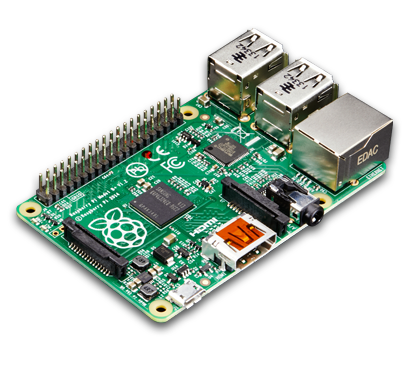
\includegraphics[scale=0.30]{../images/hardware/pi.png}
    \caption{Raspberry Pi 2B}
    \label{fig:rpi}
  \end{center}
\end{figure}

\begin{itemize}
 \item \textbf{Tarjeta de audio USB}
 \begin{itemize}
  \item Descripción: Interfaz por el cual capturamos el sonido.
  \item Especificaciónes: \url{http://www.logilink.org/showproduct/UA0078.htm}
  \item Precio: 9.37 Euros
 \end{itemize}
\end{itemize}
\begin{figure}[!h]
  \begin{center}
    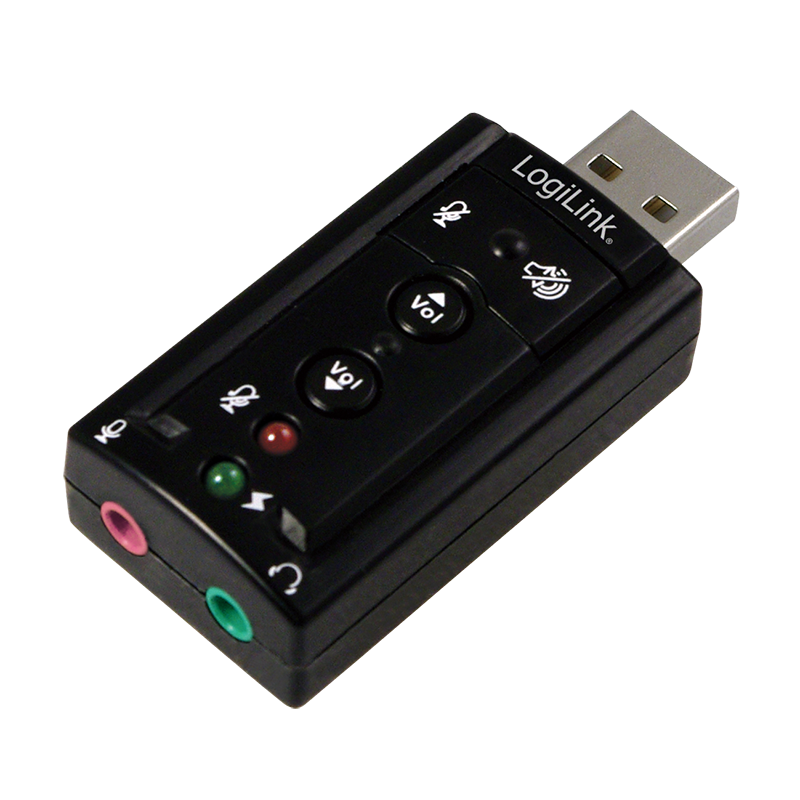
\includegraphics[scale=0.10]{../images/hardware/audiocard.png}
    \caption{Tarjeta de sonido}
    \label{fig:usbsonido}
  \end{center}
\end{figure}

\begin{itemize}
 \item \textbf{Micrófono}
 \begin{itemize}
  \item Descripción: Entrada a la interfaz de audio.
  \item Especificaciónes: \url{https://www.amazon.co.uk/Flexible-3-5mm-Microphone-Notebook-Laptop/dp/B00CRASVFC}
  \item Precio: ~5 Euros
 \end{itemize}
\end{itemize}
\begin{figure}[!ht]
  \begin{center}
    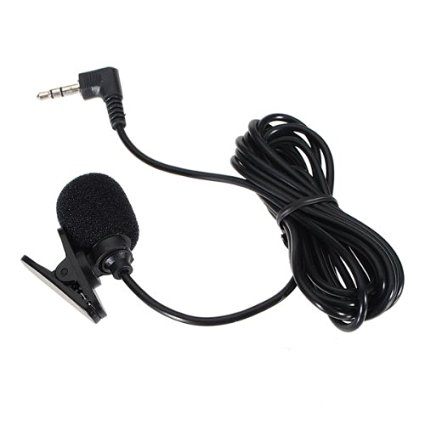
\includegraphics[scale=0.30]{../images/hardware/mic.jpg}
    \caption{Micrófono}
    \label{fig:microfono}
  \end{center}
\end{figure}

\bigskip

\begin{itemize}
 \item \textbf{Tarjeta SD (4GB)}
 \begin{itemize}
  \item Descripción: Tarjeta SD que permite la carga del SO en la Raspberry Pi.
  \item Especificaciónes: \url{https://www.amazon.com/SanDisk-Class-Memory-SDSDB-004G-B35-Change/dp/B000WQKOQM}
  \item Precio: ~12 Euros
 \end{itemize}
\end{itemize}
\begin{figure}[!ht]
  \begin{center}
    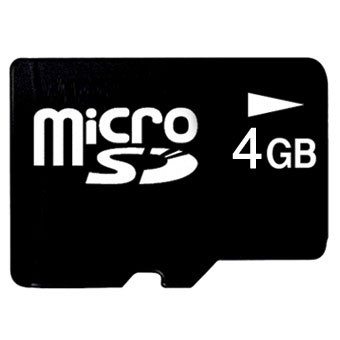
\includegraphics[scale=0.10]{../images/hardware/sd.jpg}
    \caption{Tarjeta SD}
    \label{fig:tarjetasd}
  \end{center}
\end{figure}


\begin{itemize}
 \item \textbf{Memoria USB (16GB)}
 \begin{itemize}
  \item Descripción: Memoria que contiene el SO de la Raspberry Pi.
  \item Especificaciónes: \url{http://tiendas.mediamarkt.es/p/pendrive-de-16gb-sandisk-cruzer-blade-usb-2.0-ultracompacto-en-color-negro-y-rojo-1117065}
  \item Precio: 5 Euros
 \end{itemize}
\end{itemize}
\begin{figure}[!ht]
  \begin{center}
    
\includegraphics[scale=0.05]{../images/hardware/usbdrive.jpg}
    \caption{Memoria USB}
    \label{fig:soundcard}
  \end{center}
\end{figure}

\begin{itemize}
 \item \textbf{VPS Amazon EC2}
 \begin{itemize}
  \item Descripción: Conjunto de servidores que conforman el proyecto, de tipo \textbf{t2.micro}
  \begin{itemize}
    \item 1 instancia para la plataforma IOT.
    \item 1 instancia para la base de datos de almacenamiento masivo.
    \item 1 instancia para el visualizador de datos.
    \item 1 instancia para el servidor web.
  \end{itemize}
  \item Especificaciónes: \url{https://aws.amazon.com/es/ec2/instance-types/}
  \item Precio: Este tipo de servidores son gratuitos en amazon EC2 durante un año, por lo que no existe coste computable a priori.
 \end{itemize}
\end{itemize}

Por tanto, por un total de unos 65 Euros aproximadamente podemos disponer de todo lo necesario para construir el proyecto.

\chapter{Análisis}
\label{chap4}


\subsection{Metodología}

Desde el primer momento se tiene claro que para el desarrollo del proyecto se usará el método de Desarrollo Ágil basado en iteraciones, de éste modo se van obteniendo pequeñas funcionalidades del sistema, descartando las que se consideren prescindibles.

Dentro de cada iteración tenemos unas tareas que cumplir para darla por terminada como podemos observar en la \textit{Figura \ref{fig:met_agil}}, éste método incremental permite que el desarrollo se haga sobre una base sólida evitando modificaciones que afecten al funcionamiento global de la aplicación una vez éste se encuentre en un punto avanzado del desarrollo.


\begin{figure}[!ht]
  \begin{center}
    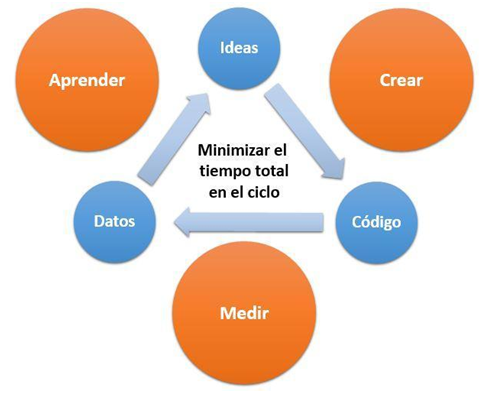
\includegraphics[scale=0.70]{../images/metodologia/agil.png}
    \caption{Metodología ágil}
    \label{fig:met_agil}
  \end{center}
\end{figure}


Por otra parte, es la manera que más natural resulta a la hora de desarrollar software pues se van completano hitos. Cada uno de ellos define una funcionalidad implementada por lo que si se desea abrir un nuevo camino \textit{(también conocidos como Fork o Roadmap)} en la aplicación tenemos varios puntos de partida evitando tener que empezar desde cero en caso de llegar a un \textit{punto muerto} en el desarrollo.

Las iteraciones se llevan acabo sobre las tareas de Implemetación, pruebas.



\section{Análisis de requisitos}

A continuación se detallan los actores implicados en el sistema, requisitos funcionales y no funcionales, requisitos de almacenamiento, casos de uso y por último los diagramas generados para el desarrollo incluyendo en éste punto los bocetos ilustrativos de interfaz de la web.

\subsection{Actores}

Los actores que hacen uso del sistema son tres, \textbf{administrador}, el \textbf{aportador de información} y \textbf{usuario visitante}.

\bigskip
El \textbf{administrador} es el encargado de mantener el correcto funcionamiento de la aplicación y sus servicios.

\bigskip
El \textbf{aportador de información} puede ser cualquier usuario que decida configurar un dispositivo para añadir información, en éste caso creando un punto que recolecte datos y los remita al sistema.

\bigskip
El \textbf{usuario visitante} puede ser cualquier persona que consulte información en la aplicación, ya sea a través de la web o através de la plataforma para consultar todos los datos almacenados (en éste último caso el usuario debe tener un mínimo de conocimientos acerca de las consultas necesarias para obtener la información).

\subsection{Requisitos funcionales}

En ésta sección se describen las funcionalidades básicas que el sistema debe cubrir para dar el problema planteado como resuelto.

\begin{itemize}
  \item \textbf{RF-1.} Mapa web:
    \begin{itemize}
      \item \textbf{RF-1.1.} Desplegar la aplicación web.
      \item \textbf{RF-1.2.} Leer datos recibidos desde los clientes.
      \item \textbf{RF-1.2.} Mostrar los datos sin necesidad de refrescar la página.
    \end{itemize}
\end{itemize}

\begin{itemize}
  \item \textbf{RF-2.} Acceso libre a la información almacenada:
    \begin{itemize}
      \item \textbf{RF-2.1.} Proveer un sistema que sea capaz de mostrar los datos almacenados y filtrarlos según la conveniencia.
      \item \textbf{RF-2.2.} Proveer un sistema que sea capaz de extraer la información consultada.
    \end{itemize}
\end{itemize}

\begin{itemize}
  \item \textbf{RF-3.} Añadir información:
    \begin{itemize}
    \item \textbf{RF-3.1.} Un usuario podrá aportar información al sistema de manera independiente y autónoma.
  \end{itemize}
\end{itemize}

\begin{itemize}
  \item \textbf{RF-3.} Identificación de vehículos:
    \begin{itemize}
    \item \textbf{RF-3.1.} Filtrar la información entrante en forma de sonido e identificar si se trata de tráfico.
    \item \textbf{RF-3.2.} Hacer una distinción según el tipo de vehículo.
    \item \textbf{RF-3.3.} Si el dispositivo recolector se queda sin conexión, debe ser capaz de seguir almacenando los datos obtenidos y enviarlos cuando le sea posible.
    \end{itemize}
\end{itemize}


\subsection{Requisitos no funcionales}

Aquí se enumeran las propiedades ligadas al desarrollo e implementación que el sistema debe cumplir.

\begin{itemize}
  \item \textbf{RNF-0.} El software de terceros usado debe ser Open Source, así como los SO usados tanto para los servidores como para la Raspberry Pi.
  \item \textbf{RNF-1.} El módulo encargado de la detección del sonido estará desarrollado en {\tt Python} por su simplicidad, las dependencias necesarias se detallarán en la sección de implementación(\ref{chap6}). Además éste módulo debe aprovechar el procesamiento en paralelo para que su funcionamiento sea óptimo.
  \item \textbf{RNF-2.} La retransmisión de datos debe ser establecida en un intervalo de tiempo mínimo para garantizar que la aplicación actúa en tiempo real.
  \item \textbf{RNF-3.} El mapa web debe mostrar la información durante un breve periodo de tiempo para no acumular señales anteriores.
  \item \textbf{RNF-4.} Siempre que sea posible se automatizarán las interacciones con cualquier elemento del sistema mediante scripts.
  \item \textbf{RNF-5.} El código de la aplicación debe estar disponible en algún sistema de control de versiones y de manera pública.
\end{itemize}

\subsection{Requisitos de almacenamiento}

La información que se almacenará en el sistema se puede dividir en dos apartados, la información almacenada que sirve para representar los datos en la web y por otra parte la información que se almacena en una base de datos diseñada para consultas de datos masivas, que aunque tienen elementos similares difieren en algunos aspectos.

\begin{itemize}
  \item \textbf{RA-1.} Almacenamiento para la web.
  \begin{itemize}
    \item Timestamp de la señal recibida.
    \item Coordenadas de la señal recibida.
    \item Valor (numérico) de la señal recibida.
  \end{itemize}
  \item \textbf{RA-2.} Almacenamiento de datos masivo.
  \begin{itemize}
    \item Localización.
    \item Timestamp.
    \item Id del dispositivo.
    \item Valor de la señal.
  \end{itemize}
\end{itemize}

Obsérvese que no se almacena ningún dato personal luego a efectos prácticos, los artículos 7 y 8 de la LOPD en los que se detalla el tipo de datos de carácter sensible que hay que preservar con especial atención no tienen aplicación sobre RSMap.


\newpage

\section{Casos de uso}

Debido a que RSMap es un servicio para proveer y aportar información, los casos de uso quedan simplificados de manera que la mayor parte de ellos hacen referencia a la aportación/consulta de datos.

\subsection{Descripción de actores}

\begin{itemize}
  \item \textbf{A-1.} Administrador.
  \begin{itemize}
   \item Descripción: Es el responsable del correcto funcionamiento de la aplicación.
   \item Tareas: Administración, mantenimiento y actualización de todos los elementos que conforman el sistema.
  \end{itemize}

  \item \textbf{A-2.} Usuario aportador de información.
  \begin{itemize}
   \item Descripción: Persona que se dispone a configurar un dispositivo para añadir información al sistema.
   \item Comentarios: Debe tener un conocimiento mínimo en sistemas operativos, concretamente en Linux (Raspberry Pi) para configurar el dispositivo y proceder a remitir información.
  \end{itemize}

  \item \textbf{A-2.} Usuario visitante.
  \begin{itemize}
   \item Descripción: Persona que se dispone a consultar los datos que almacena el sistema.
   \item Comentarios: Para la consulta de datos mediante la web no necesita ningún conocimiento, para la consulta en el almacenamiento masivo tal vez sea necesario tener conocimientos básicos en consultas. En cualquier caso se proveerán consultas predefinidas cuyos parámetros sean totalmente configurables.
  \end{itemize}
\end{itemize}

\subsection{Casos de uso}

\begin{itemize}
  \item \textbf{CU-1.} Desplegar servicio Web RSMap.
  \begin{itemize}
    \item Actores: Administrador.
    \item Tipo: Primario, esencial.
    \item Referencias:
    \item Precondición: Disponer de los ficheros de GitHub para lanzarla y una correcta configuración de puertos.
    \item Postcondición: Se ejecuta el servidor web de RSMap.
    \item Autor: \autor.
    \item Versión: 1.0.
    \item Propósito: Levantar una instancia de la web de RSMap.
    \item Resumen: El desarrollador puede actualizar la aplicación desde GitHub y lanzarla de manera fácil con nuevas funcionalidades.
  \end{itemize}
\end{itemize}
\begin{table}[!ht]
  \begin{center}
    \begin{tabular}{|l|l|l|l|}
      \hline
      \multicolumn{4}{|c|}{{\bf Caso de uso 1}}
      \\ \hline
      \multicolumn{2}{|c|}{{\bf Actor}} & \multicolumn{2}{c|}{{\bf Sistema}}
      \\ \hline
      {\it 1} &
      \begin{tabular}[c]{@{}l@{}}
        Administrador: descarga el\\
        repositorio de RSMap y\\
        lanza la aplicación web.
      \end{tabular} &
      &
      \\ \hline
      &
      &
      {\it 2} &
      \begin{tabular}[c]{@{}l@{}}
        El sistema sobre el que se  \\
        instala levanta un\\
        servicio web que contiene RSMap.\\
      \end{tabular}
      \\ \hline
    \end{tabular}
    \caption{Secuencia de CU-1}
    \label{table:cu_1}
  \end{center}
\end{table}

\begin{table}[!ht]
  \begin{center}
\begin{tabular}{|l|l|}
\hline
\multicolumn{2}{|c|}{{\bf Curso alterno}}
\\ \hline
{\it 2b} &
\begin{tabular}[c]{@{}l@{}}
  Si el servidor está funcionando, no se ejecuta \\
  la nueva instancia de la web.
\end{tabular}\\
\hline
\end{tabular}
\caption{Curso alterno de CU-1.}
\label{table:ca_cu_1}
  \end{center}
\end{table}

\newpage

\begin{itemize}
  \item \textbf{CU-2.} Configurar los clientes de RSMap.
  \begin{itemize}
    \item Actores: Administrador.
    \item Tipo: Primario, esencial.
    \item Referencias:
    \item Precondición: Disponer de los servidores necesarios para enviar la información.
    \item Postcondición: Los clientes remitirán los datos a donde el administrador desee.
    \item Autor: \autor.
    \item Versión: 1.0.
    \item Propósito: Permitir que un administrador defina nuevas localizaciones de almacenamiento.
    \item Resumen: El desarrollador puede actualizar la aplicación desde GitHub y ponerla a disposición de futuros usuarios aportadores de información.
  \end{itemize}
\end{itemize}
\begin{table}[!ht]
  \begin{center}
    \begin{tabular}{|l|l|l|l|}
      \hline
      \multicolumn{4}{|c|}{{\bf Caso de uso 2}}
      \\ \hline
      \multicolumn{2}{|c|}{{\bf Actor}} & \multicolumn{2}{c|}{{\bf Sistema}}
      \\ \hline
      {\it 1} &
      \begin{tabular}[c]{@{}l@{}}
        Administrador: descarga el\\
        repositorio de RSMapPi y\\
        lo configura con nuevos\\
        parámetros.
      \end{tabular} &
      &
      \\ \hline
      &
      &
      {\it 2} &
      \begin{tabular}[c]{@{}l@{}}
        La nueva configuración de\\
        los clientes permite enviar\\
        información a el destino\\
        seleccionado por el\\
        administrador\\.
      \end{tabular}
      \\ \hline
    \end{tabular}
    \caption{Secuencia de CU-2}
    \label{table:cu_1}
  \end{center}
\end{table}

\newpage

  \item \textbf{CU-3.} Consulta de datos mediante la web.
  \begin{itemize}
    \item Actores: Usuario visitante.
    \item Tipo: Primario, esencial.
    \item Referencias:
    \item Precondición: La aplicación web debe estar en funcionamiento.
    \item Postcondición: Se muestran identificadores en los lugares en los que se encuentra un dispositivo receptor y detecta tráfico.
    \item Autor: Cualquier usuario que acceda a la plataforma.
    \item Versión: 1.0.
    \item Propósito: Que el usuario tenga conocimiento de por que zonas existe tráfico.
    \item Resumen: El usuario entra en la web y puede ver el tráfico en tiempo real.
    \begin{table}[!ht]
      \begin{center}
	\begin{tabular}{|l|l|l|l|}
	  \hline
	  \multicolumn{4}{|c|}{{\bf Caso de uso 3}}
	  \\ \hline
	  \multicolumn{2}{|c|}{{\bf Actor}} & \multicolumn{2}{c|}{{\bf Sistema}}
	  \\ \hline
	  {\it 1} &
	  \begin{tabular}[c]{@{}l@{}}
	    Usuario: accede en la web\\
	    para visualizar el tráfico\\
	  \end{tabular} &
	  &
	  \\ \hline
	  &
	  &
	  {\it 2} &
	  \begin{tabular}[c]{@{}l@{}}
	    Muestra los marcas en los lugares \\
        en los que existe tráfico \\
        en ese momento. \\
	  \end{tabular}
	  \\ \hline
	\end{tabular}
	\caption{Secuencia de CU-3}
	\label{table:cu_2}
      \end{center}
    \end{table}

\begin{table}[!ht]
  \begin{center}
\begin{tabular}{|l|l|}
\hline
\multicolumn{2}{|c|}{{\bf Curso alterno}}
\\ \hline
{\it 2b} &
\begin{tabular}[c]{@{}l@{}}
  Si el no exiten dispositivos retransmitiendo\\
  la web informa al usuario.
\end{tabular}\\
\hline
\end{tabular}
\caption{Curso alterno de CU-3.}
\label{table:ca_cu_2}
  \end{center}
\end{table}

\newpage

  \item \textbf{CU-4.} Consulta de datos masivos.
  \begin{itemize}
    \item Actores: Usuario visitante.
    \item Tipo: Primario, esencial.
    \item Referencias:
    \item Precondición: La aplicación web debe estar en funcionamiento y la base de datos debe contener registros.
    \item Postcondición: Se muestran los datos según la consulta enviada.
    \item Autor: Cualquier usuario que acceda a la plataforma.
    \item Versión: 1.0.
    \item Propósito: Que el usuario tenga libre acceso a la información recopilada por los dispositivos que agregan información.
    \item Resumen: El usuario entra en la web y puede consultar los datos almacenados bajo las condiciones que el desee.
    \begin{table}[!ht]
      \begin{center}
    \begin{tabular}{|l|l|l|l|}
      \hline
      \multicolumn{4}{|c|}{{\bf Caso de uso 4}}
      \\ \hline
      \multicolumn{2}{|c|}{{\bf Actor}} & \multicolumn{2}{c|}{{\bf Sistema}}
      \\ \hline
      {\it 1} &
      \begin{tabular}[c]{@{}l@{}}
        Usuario: accede en la web\\
        y lanza una consulta \\
      \end{tabular} &
      &
      \\ \hline
      &
      &
      {\it 2} &
      \begin{tabular}[c]{@{}l@{}}
        Devuelve todas las entradas \\
        que cumplen las condiciones \\
        de la consulta. \\
      \end{tabular}
      \\ \hline
    \end{tabular}
    \caption{Secuencia de CU-4}
    \label{table:cu_3}
      \end{center}
    \end{table}
  \end{itemize}

  \begin{table}[!ht]
    \begin{center}
  \begin{tabular}{|l|l|}
  \hline
  \multicolumn{2}{|c|}{{\bf Curso alterno}}
  \\ \hline
  {\it 2b} &
  \begin{tabular}[c]{@{}l@{}}
    Si no existen datos en base a la consulta \\
    el sistema no devuelve nada y se muestra un error.
  \end{tabular}\\
  \hline
  \end{tabular}
  \caption{Curso alterno de CU-4.}
  \label{table:ca_cu_1}
    \end{center}
  \end{table}

\newpage

  \item \textbf{CU-5.} Añadir nuevos dispositivos.
  \begin{itemize}
    \item Actores: Aportador de información.
    \item Tipo: Primario, esencial.
    \item Referencias:
    \item Precondición: Tiene un dispositivo capaz de remitir información al sistema.
    \item Postcondición: Los datos que remitidos quedan guardados en el sistema.
    \item Autor: Administrador, Usuario Aportador.
    \item Versión: 1.0.
    \item Propósito: Que cualquier usuario pueda aportar información al sistema.
    \item Resumen: El usuario se descarga desde GitHub el cliente y lo ejecuta para enviar información del tráfico en su localización.
    \begin{table}[!ht]
      \begin{center}
	\begin{tabular}{|l|l|l|l|}
	  \hline
	  \multicolumn{4}{|c|}{{\bf Caso de uso 5}}
	  \\ \hline
	  \multicolumn{2}{|c|}{{\bf Actor}} & \multicolumn{2}{c|}{{\bf Sistema}}
	  \\ \hline
	  {\it 1} &
	  \begin{tabular}[c]{@{}l@{}}
	    Usuario: se descarga el cliente\\
	    y lo configura para el envío\\
	  \end{tabular} &
	  &
	  \\ \hline
	  &
	  &
	  {\it 2} &
	  \begin{tabular}[c]{@{}l@{}}
	    Almacena los datos remitidos \\
        por el usuario aportador. \\
	  \end{tabular}
	  \\ \hline
	\end{tabular}
	\caption{Secuencia de CU-5}
	\label{table:cu_4}
      \end{center}
    \end{table}
  \end{itemize}

\end{itemize}

\newpage
\section{Diagramas}
\subsection{Diagrama de paquetes}

En este diagrama podemos observar las dependencias que existen entre los distintos paquetes del sistema y como el paquete \textbf{IOT} es el elemento central sobre el que se apoyan los demás. El paquete \textbf{Raspberry Pi} es dependiente del paquete de \textbf{IOT} debido a que \textbf{IOT} es el encargado de definir como los clientes van a escribir en el almacenamiento masivo. A su vez el paquete \textbf{RSMap web} es dependiente de \textbf{Raspberry Pi} debido a que las señales de vehículos se mandarán directamente a la plataforma web gracias a la \textbf{API REST}.

Por otra parte tenemos el paquete \textbf{Visualizador} el cual usa al paquete \textbf{Almacenamiento masivo} para proveerse de información que mostrar. Por último \textbf{Almacenamiento masivo} es dependiente de \textbf{IOT} debido a que los esquemas (estructura de almacenamiento) se definen en \textbf{IOT} y éste se encarga de definirlas en el \textbf{Almacenamiento masivo}.

\begin{figure}[!ht]
  \begin{center}
    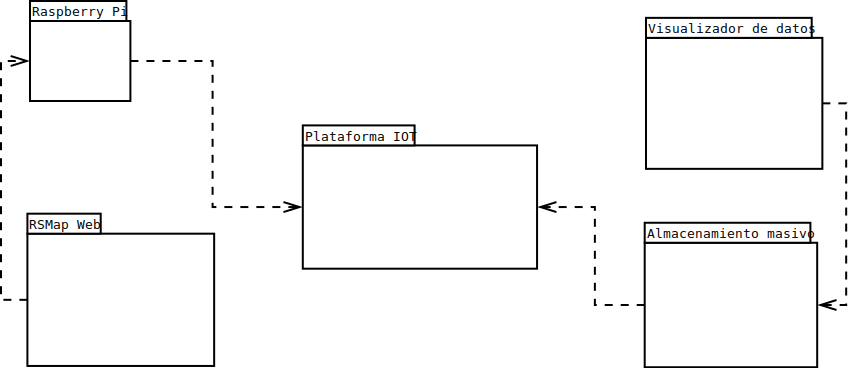
\includegraphics[scale=0.50]{../images/diag_plan/paquetes.png}
    \caption{Diagrama de paquetes}
    \label{fig:paquetes}
  \end{center}
\end{figure}

\newpage

\subsection{Diagrama arquitectónico}

En ésta sección se detallan los elementos de la estructura que compondrá la aplicación. Debido a que los dispositivos receptores \textbf{(Raspberry pi)} poseen una estructura interna la cual merece atención se han detallado por separado el diagrama de los receptores \textit{(Figura \ref{fig:ar_rpi})} y el del sistema completo \textit{(Figura \ref{fig:ar_rsmap})}.

\bigskip

El sistema recibirá la entrada de audio mediante un micrófono, tras ésto el módulo encargado de recolectar los datos efectuará un filtrado previo evitando así analizar datos innecesarios de ésta manera minimizamos la sobrecarga del dispositivo. Tras ésto se procede a analizar los datos que han pasado el primer filtro. Por último se envían los datos con los resultados a los distintos sistemas de almacenamiento que se detallan en el siguiente diagrama.

\bigskip

\begin{figure}[!ht]
  \begin{center}
  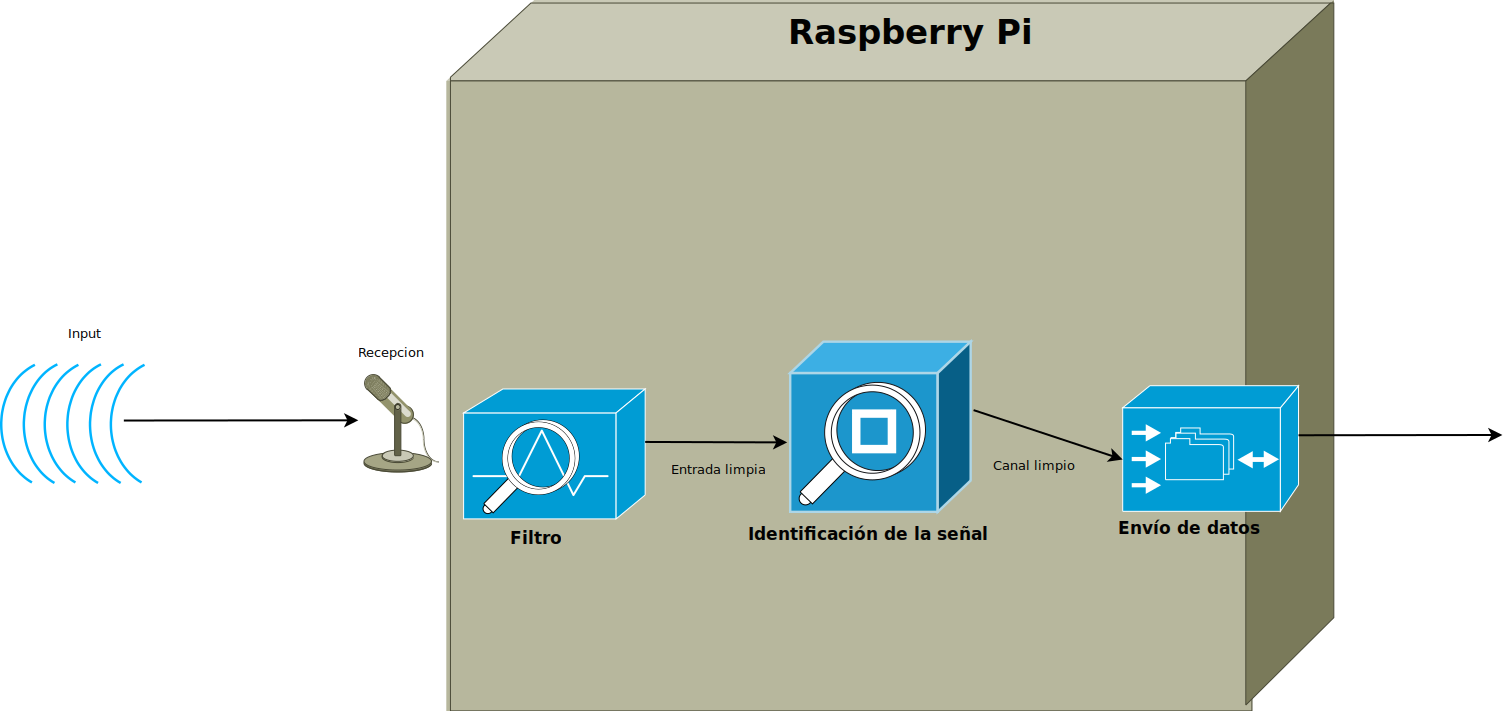
\includegraphics[scale=0.25]{../images/diag_plan/diag_arqu_pi.png}
  \caption{Arquitectura Raspberry Pi}
  \label{fig:ar_rpi}
  \end{center}
\end{figure}

\newpage

Ahora se muestra cual será la estructura en conjunto de todos los elementos que conforman \textbf{RSMap.}


Tras haber analizado el comportamiento de los dispositivos receptores, el siguiente elemento a destacar es la plataforma IOT, la manera de transmitir la información según la configuración establecida, en la que se detalla a donde tienen que remitir los dispositivos la información así como los propios modelos de datos. Los receptores harán uso de ésto para enviar la información a \textbf{Almacenamiento masivo}.

Por otra parte, también realizarán envíos a el servidor web indicando cuando pasa un vehículo por la localización en la que se encuentren, el cual atenderá las peticiones de los clientes que soliciten acceder a RSMap.

Como último elemento nos queda \textbf{Visualizador}, que actúa a modo de Notebook y es el encargado de realizar las consultas que el usuario defina a \textbf{Almacenamiento masivo} para poder acceder a los datos que han almacenado los dispositivos receptores.

\begin{figure}[!ht]
  \begin{center}
  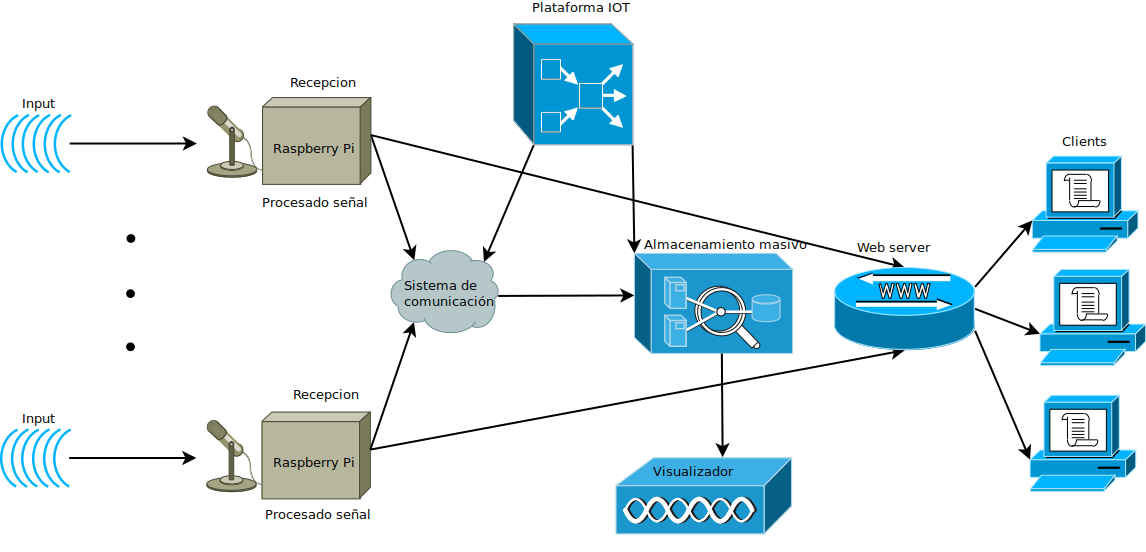
\includegraphics[scale=0.35]{../images/diag_plan/diag_arqu.png}
  \caption{Arquitectura de RSMap}
  \label{fig:ar_rsmap}
  \end{center}
\end{figure}

\newpage

\subsection{Diagrama de clases}

En éste diagrama se presentan los elementos de RSMap como clases y cuales serían los métodos y campos ideales para cada uno de ellos.

\begin{figure}[!ht]
  \begin{center}
  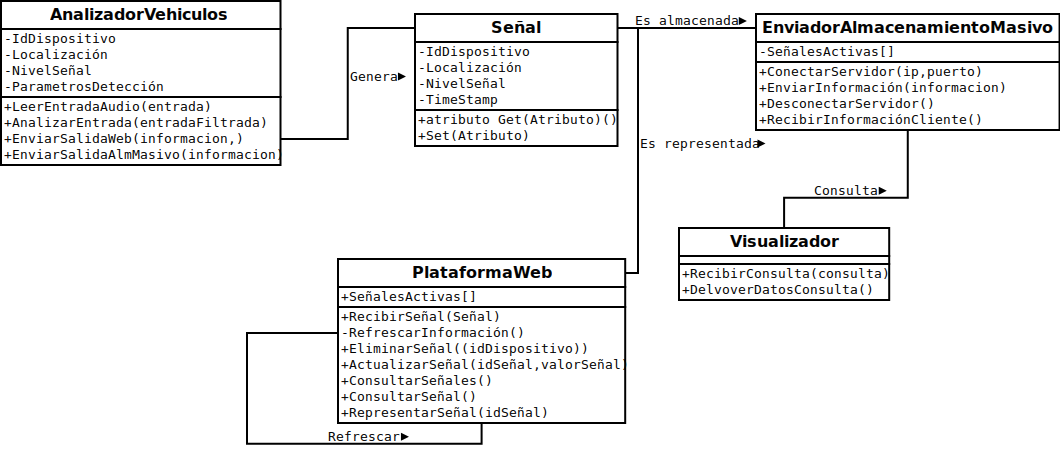
\includegraphics[scale=0.4]{../images/diag_plan/clases.png}
  \caption{Diagrama de clases}
  \label{fig:ar_rsmap}
  \end{center}
\end{figure}

\newpage

\subsection{Diagramas de casos de uso}

Ahora detallaremos de qué manera pueden interactuar los distintos actores con el sistema. A modo de vista general se proporciona un diagrama de Caso de uso global.

\begin{figure}[!ht]
  \begin{center}
    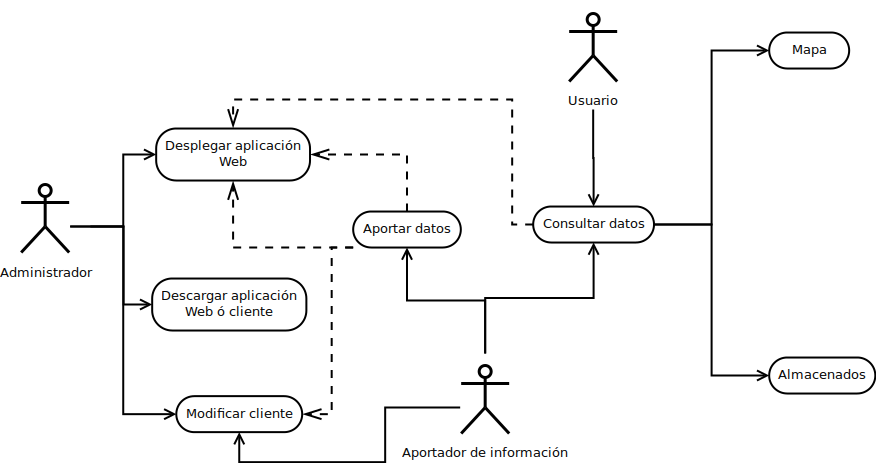
\includegraphics[scale=0.45]{../images/diag_plan/cu_gen.png}
    \caption{Caso de uso general}
    \label{fig:cu_admin}
  \end{center}
\end{figure}



El administrador tiene capacidad para realizar actividades de mantenimiento y chequeo de los parámetros usados, así como generar nuevas configuraciones.
\begin{figure}[!ht]
  \begin{center}
    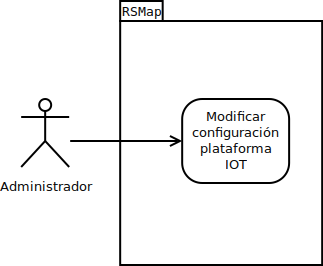
\includegraphics[scale=0.45]{../images/diag_plan/cu_admin.png}
    \caption{Caso de uso del administrador}
    \label{fig:cu_admin}
  \end{center}
\end{figure}

\newpage

En segundo lugar tenemos el usuario que puede consultar los datos bien sea mediante el mapa web, el cual sólo indica señales en los puntos en los que pasen vehículos, mientras que mediante el visualizador de datos masivos podrá consultar el conjunto total de información almacenada.

\begin{figure}[!ht]
  \begin{center}
  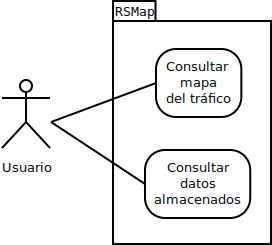
\includegraphics[width=0.45\textwidth]{../images/diag_plan/cu_usuario.png}
  \caption{Caso de uso del usuario}
  \label{fig:cu_usuario}
  \end{center}
\end{figure}

Por último el usuario aportador podrá bajarse el código fuente desde GitHub y podrá ejecutarlo para enviar la información a RSMap. Como se trata de una especialización del Usuario, se da por entendido que también tendrá acceso a los datos.

\begin{figure}[!ht]
  \begin{center}
  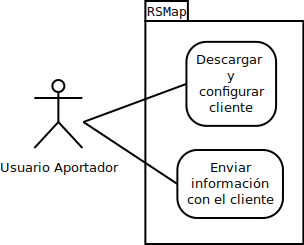
\includegraphics[width=0.45\textwidth]{../images/diag_plan/cu_usuario_aportador.png}
  \caption{Caso de uso del usuario aportador}
  \label{fig:cu_uaportador}
  \end{center}
\end{figure}

\newpage


\subsection{Diagramas de secuencia}

Ahora se detallan los pasos de forma generalizada que cada tipo de usuario realiza y qué efectos desencadenan sobre el sistema.

\begin{figure}[!h]
  \begin{center}
  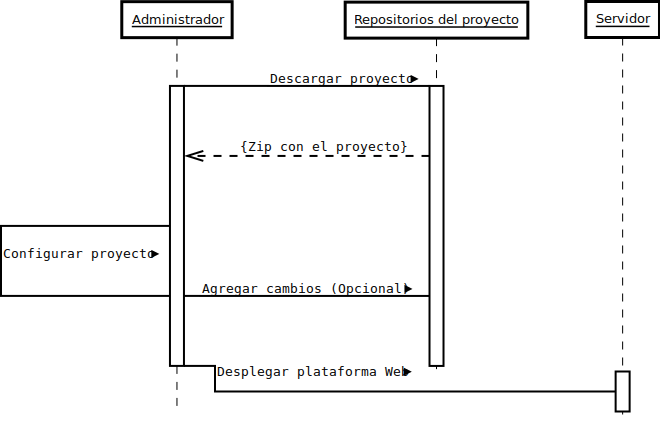
\includegraphics[scale=0.45]{../images/diag_plan/seq_admin.png}
  \caption{Diagrama de secuencia del Administrador}
  \label{fig:ar_rsmap}
  \end{center}
\end{figure}

\newpage

\begin{figure}[!h]
  \begin{center}
  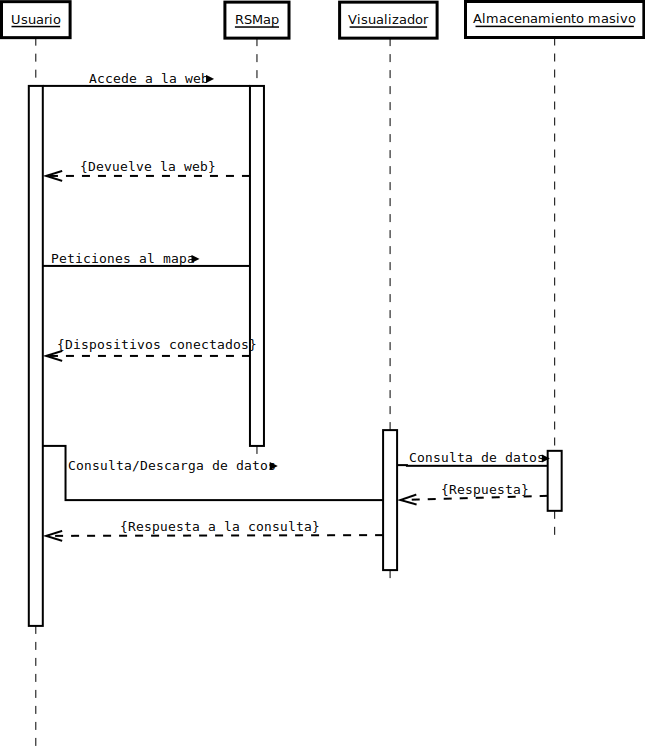
\includegraphics[scale=0.5]{../images/diag_plan/seq_user.png}
  \caption{Diagrama de secuencia del Usuario}
  \label{fig:ar_rsmap}
  \end{center}
\end{figure}

\newpage

\begin{figure}[!h]
  \begin{center}
  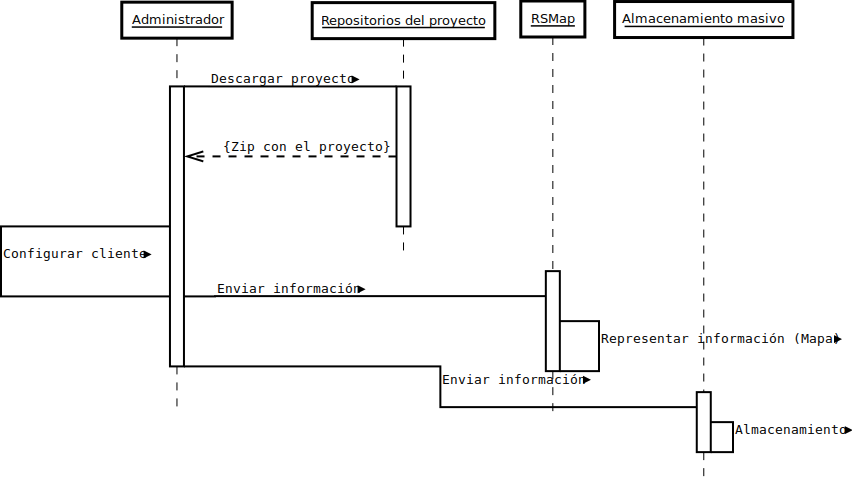
\includegraphics[scale=0.45]{../images/diag_plan/seq_user_ap.png}
  \caption{Diagrama de secuencia del Usuario Aportador}
  \label{fig:ar_rsmap}
  \end{center}
\end{figure}

\newpage

\subsection{Diagramas de interfaz}

Aquí se presentan dos pequeños esbozos de una aproximación a la interfaz de la web, no se ha entrado en mucho nivel de detalle debido a que la idea es usar una plantilla de Bootstrap y adaptarla a las necesidades, en cualquier caso el aspecto deberá asemejarse al ilustrado en la \textit{Figura \ref{fig:i1}} para la página principal y para la página del mapa el de la \textit{Figura \ref{fig:i2}}.

\begin{figure}[!ht]
  \begin{center}
  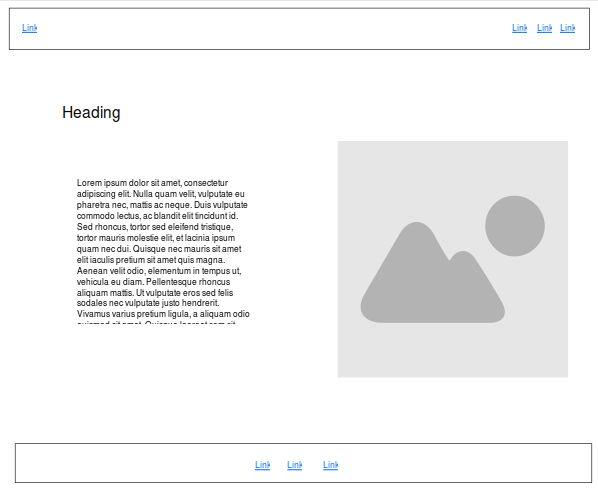
\includegraphics[scale=0.6]{../images/diag_plan/ui_general.png}
  \caption{Boceto de la página principal}
  \label{fig:i1}
  \end{center}
\end{figure}

\newpage

\begin{figure}[!ht]
  \begin{center}
  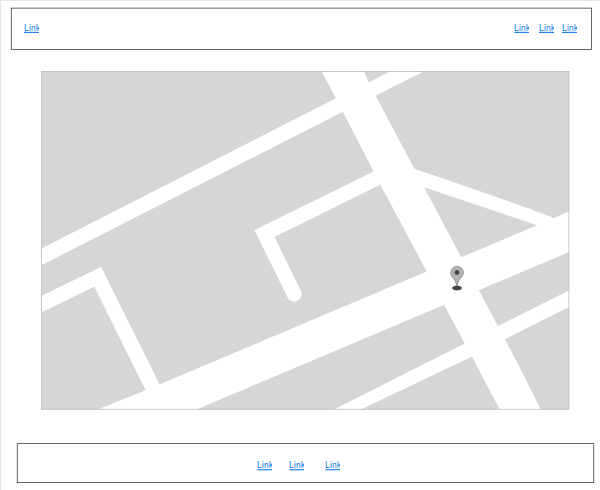
\includegraphics[scale=0.65]{../images/diag_plan/ui_mapa.png}
  \caption{Boceto de la página del mapa}
  \label{fig:i2}
  \end{center}
\end{figure}

\chapter{Diseño}

Éste apartado muestra una visión simplificada de como funciona la aplicación, será en la sección de implementación donde se completen los aspectos restantes cuya explicación resulta más fácil valiéndose del código usado además el porqué de la elección de las tecnologías con las que se llevan a cabo las tareas.

\section{Diseño del dispositivo receptor}

El dispositivo receptor tendrá instalado y en continua ejecución el módulo de reconocimiento de vehículos. Los elementos hardware requeridos se detallaron en la sección \textit{presupuesto}.

\section{Diseño del módulo de reconocimiento de vehículos}
El lenguaje usado para la recepción de sonido será {\tt Python 3} debido a la facilidad de uso y el número de librerías que presenta. Por otra parte
El módulo principal estará compuesto de dos funciones usando como base un patrón típico en sistemas concurrentes, el  modelo de productor-consumidor. Ésto nos permitirá trabajar con dos hebras independientes (pero pertenecientes al mismo proceso) las cuales trabajan sobre una cola en la que la hebra productora va introduciendo los valores numéricos obtenidos por el micrófono mientras que el consumidor va extrayendo los mismos de la cola para su análisis, el cual se detalla en la subsección Desarrollos algorítmicos.

Una vez el consumidor ha concretado que la información recibida es indicador de que un vehículo ha pasado tiene dos tareas:

\begin{itemize}
  \item Enviar la información a la web mediante una petición HTTP que incluya un \textit{payload} con la información relativa al dispositivo por ejemplo latitud, longitud, id del dispositivo y nivel de la señal. Las peticiones serán aceptadas en el servidor web gracias a una api REST que atiende las peticiones de éste tipo.
  \item Transmitir la información al almacenamiento masivo mediante el soporte que nos provea la plataforma IOT KAA. La forma de proceder aquí es dependiente de cómo se interactúe con la plataforma por tanto los detalles de como el dispositivo envía la información en éste punto serán vistos en el sección de implementación.
\end{itemize}

\subsection{Estructuras de datos en el dispositivo receptor}
La estructura de datos más remarcable en éste módulo es la cola, sin duda es el elemento más apropiado para la recopilación y extracción de datos de manera simultánea. Además las colas en python están diseñadas para solventar problemas de tipo concurrente de manera interna.

\bigskip

Para transmitir la información a la web se usarán diccionarios de tipo \textit{'clave':valor} en formato JSON cuyo tamaño reducido los hace ideales para enviarlos de manera recurrente.

\bigskip

Por otra parte tenemos la estructura de datos Señal, que almacenará toda la información necesaria para ser almacena/representada en RSMap. Se hace uso de ella en en el módulo de envío proporcionado por KAA, en la base de datos de almacenamiento masivo Apache Cassandra y en los modelos definidos en Django para la web.

\subsection{Desarrollos algorítmicos}

A continuación se explica cuál es la forma de proceder a la identificación de un vehículo mediante el sonido recogido, por eso es imprescindible hablar del análisis de señales además del algoritmo usado.

\begin{itemize}
  \item \textbf{Digitalización de señales: }

    \begin{itemize}
      \item Para obtener una señal discreta a partir de una señal continua, es decir, para convertir los datos del dominio del tiempo al dominio de la frecuencia nos valdremos de la transformada rápida de Fourier (FFT).
      \item Con los valores discretizados procedemos a multiplicarlos por una ganancia configurable mediante una constante, que ayudará a aumentar la señal o disminuirla dependiendo del tipo de micrófono y tarjeta de audio que tengamos. Los valores serán contabilizados en forma de bloques (que están definidos en milisegundos), se suman los valores que pertenecen a un mismo bloque descartando aquellos que no entren dentro del rango de cuantización establecido que nos indique que se trata de un vehículo. Éste valor final es puesto en la cola sobre la que la hebra consumidora va extrayendo datos.
    \end{itemize}

  \item \textbf{Identificación de vehículos:} Una vez tenemos la suma de los valores para un bloque, en primer lugar comprobamos que la suma de ese bloque alcanza un nivel mínimo, éste nivel dependerá de las condiciones en las que se encuentre el dispositivo receptor. Por ejemplo, no es lo mismo que se encuentre situado en el primer piso de un edificio que en un tercero.

  Una vez tenemos filtrados los valores que superan ese mínimo es momento de contar cuantos bloques seguidos se obtienen por encima de una cota mínima de bloques. Al igual que hemos definido la cota mínima para considerar que existe un nivel de sonido perteneciente a un vehículo debemos definir el número de bloques consecutivos que necesitamos para considerar que un vehículo ha pasado y éste valor será dependiente de igual modo de las características de la carretera ya que el número de bloques necesarios para la identificación está estrictamente relacionado con la velocidad de los vehículos que circulan por la calle, es decir, cuanta más velocidad lleven menos bloques serán necesarios para proceder a la identificación del vehículo.

  El valor de cada bloque válido (que supera la cota), es almacenado en una cola, cuando el número de bloques es suficiente para concretar que un vehículo ha pasado los valores almacenados en la cola se mandan a la base de datos de almacenamiento masivo así como a la API y ya estarán listos para su visualización.

  Para ilustrarlo con un ejemplo nos valdremos de la \textit{figura 5.1}.

  Cuando el vehículo pasa dentro del rango de captura del micrófono empiezan a contabilizarse los bloques con un valor superior a la cota definida desde \textbf{B1} hasta \textbf{BN}. Si tenemos un número de bloques válido contabilizaremos que ha pasado un vehículo. Si el número de bloques se ve interrumpido por 'silencio' o sonido por debajo de la cota, la contabilización de bloques se reinicia y en la cola de envío son descartados todos los elementos pertenecientes a los bloques consecutivos anteriores.
\end{itemize}
\begin{figure}[!ht]
  \begin{center}
    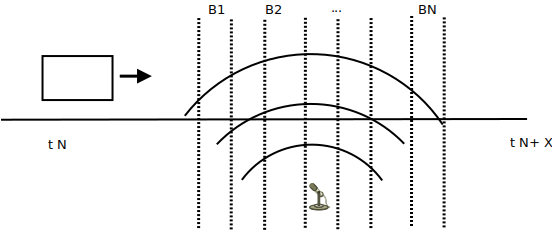
\includegraphics[scale=0.50]{../images/sound/soun_detect.png}
    \caption{Proceso de reconocimiento}
    \label{fig:recogn}
  \end{center}
\end{figure}

\newpage

\section{Almacenamiento de información}

La información será enviada desde los dispositivos recolectores hasta el servidor que contiene la base de datos de Apache Cassandra que se encontrará instalada en una instancia propia para garantizar que todos los recursos de la máquina se dedican a atender las peticiones de almacenamiento. Por otra parte las peticiones HTTP se realizarán mediante ficheros JSON contra una API Rest construida bajo Django-Rest-Framework

Ésta base de datos será de tipo NoSQL debido a que no se requiere ningún tipo de jerarquía sobre los datos y tampoco se precisa una estricta integridad de los mismos ni operaciones de tipo atómico.

\bigskip

Por otra parte tenemos la base de datos de la que hará uso la web de RSMap para la representación en el mapa. Al ser datos de caracter temporal cuyo formato no mantiene ningún tipo de jerarquía relacional se usará SQLite.

\section{Representación de información}

Éste módulo trabaja con Apache Zeppelin que también se encontrará en un servidor externo a los demás. En la configuración se establecerá la conexión hacia el servidor de almacenamiento masivo y a partir de ahí, se podrán lanzar consultas para obtener datos.

\newpage

\section{Diseño del portal web}

El portal estará desarrollao con el framework Django, el cual hace uso del paradigma modelo Vista-Controlador por lo que tendremos por una parte la parte lógica o Backend y por otro lado la parte visual o Frontend. Tendrá la siguiente estructura de archivos y directorios:

\begin{itemize}
  \item \textbf{resources}: archivos complementarios (no necesarios).
  \item \textbf{rsmap}: contiene el proyecto principal de la aplicación en el que se definen los parámetros generales.
  \begin{itemize}
      \item \textit{urls.py}: definicióno de las rutas globales de la web.
      \item \textit{wsgi.py}: configuración de despliegue.
      \item \textit{settings.py}: archivo de configuración general.
  \end{itemize}
  \item \textbf{rsmapweb}: contiene la aplicación web y la API rest.
  \begin{itemize}
    \item \textbf{templates}: contiene las plantillas html de la web.
    \begin{itemize}
      \item \textit{(index.html)} alberga la página principal.
      \item \textit{(map.html)} representa la página que contiene el mapa.
    \end{itemize}
    \item \textbf{static}: contiene los archivos estáticos de la web (css, fuentes, etc).
      \begin{itemize}
        \item \textbf{js}: es el directorio más importante ya que contiene el script encargado de interactuar con el mapa \textit{(rsmapMapUpdater.js)}
      \end{itemize}
    \item \textit{admin.py} archivo para configurar la administración del portal.
    \item \textit{apps.py}: archivo en el que se configura las aplicaciones instaladas de la web.
    \item \textit{models.py}: modelos de datos que serán usados.
    \item \textit{urls.py}: definicióno de las rutas de la aplicación y la API rest.
    \item \textit{serializers.py}: define qué información devolverá al API rest.
    \item \textit{views.py}: definición de vistas
  \end{itemize}
    \item \textit{manage.py}: encargado de ejecutar tareas de lanzar la aplicación además de actualizar los modelos de datos en la base de datos.
    \item \textit{requirements.txt}: dependencias necesarias para la aplicación.
    \item \textit{Makefile}: contiene la automatización de las tareas más comunes de la aplicación.
\end{itemize}

En lo que a la parte visual se refiere, se usará Bootstrap para garantizar un diseño adaptativo al formato de dispositivo desde el cual se consulte la información.

\subsection{Diseño de la api REST}

La api estará integrada dentro de Django gracias al módulo Django-Rest-Framework, es por éste motivo por lo que se desarrolla dentro de la sección \textit{Diseño del portal web}.

\bigskip

Una API se caracteriza por ofrecer una serie de URL's sobre las que realizar peticiones HTTP de diverso tipo como podrían ser POST, GET, PATCH, PUT o DELETE entre otras.

Éstas peticiones contienen un \textit{payload} con la información necesaria para que, una vez recibida la petición, la API se encarge internamente de interactuar con los modelos creados en Django que afecten a la misma.

\bigskip

Las rutas tendrán una estructura similar a la siguiente:

\begin{itemize}
  \item \textbf{Consultar listado o añadir dispositivos al mismo:}

  \url{http://urlweb/api/signals/}

  Devolverá un JSON con los dispositivos que están retransmitiendo información en ese momento (GET), además ésta ruta debe permitir registrar nuevos dispositivos (POST) por lo que los métodos permitidos en ella serán POST y GET.

  \item \textbf{Actualizar estado de dispositivo:}

  \url{http://urlweb/api/signal/signalID}

  Con ésta url podremos obtener los detalles de esta señal en concreto (GET), actualizar el estado de una señal (PATCH) o eliminarla en consecuencia de que el dispositivo deje de retransmitir (DELETE), de ésta manera el servidor web no tendrá que descargar continuamente el JSON de todos los dispositivos para representarlo en el mapa si no únicamente aquellos que se encuentren retransmitiendo en ese momento. Por tanto los métodos permitidos para ésta URL serán GET, PATCH y DELETE.
\end{itemize}

\chapter{Implementación}

A continuación se detallan la instalación, configuración así como el desarrollo de los elementos que componenen el sistema. A modo de resumen los puntos serán los siguientes:

\begin{itemize}
	\item Descripción de las tecnologías seleccionadas.
	\item Instalación y configuración de Raspberry Pi.
	\item Instalación y configuración de KAA.
	\item Instalación y configuración de Apache Cassandra.
	\item Desarrollo del módulo de detección de vehículos.
	\item Desarrollo de la plataforma web.
	\item Instalación y configuración de Apache Zeppelin.
\end{itemize}

\newpage

\section{ Descripción de las tecnologías seleccionadas}

Éste apartado detalla las tecnologías seleccionadas así como las que finalmente fueron descartadas.

A lo largo del desarrollo del proyecto el diseño ha ido cambiando progresivamente debido a que el número de elementos que lo componen deben cohesionarse para trabajar sobre la solución, siendo éste uno de los mayores problemas encontrados ya que al elegir una tecnología se deben desarrollar una serie de pruebas para confirmar que es la óptima de cara al diseño final.

\newpage

\subsection{Plataforma IOT}

Éste aspecto ha sio uno de los más relevantes, el cual ha marcado el funcionamiento final de la aplicación. Existen muchas alternativas debido al auge de IOT no obstante la plataforma debía cumplir una serie de premisas enumeradas a continuación:

\begin{itemize}
    \item \textbf{Open Source: } para mantener el licenciamiento de la aplicación final.
    \item \textbf{Independiente: } esto es, debe ser un sistema instalable en un servidor propio sin necesidad de depender de servidores de terceros.
    \item \textbf{Soporte para Raspberry Pi: } es obvio que debe poderse integrar con nuestro dispositivo receptor.
    \item \textbf{Número de dispositivos ilimitado: } esto nos permitirá cumplir con el requisito de que cualquiera pueda proveer datos a la aplicación.
    \item \textbf{Documentación: } es un elemento importante, más aún, cuando se desconoce la materia.
\end{itemize}

El abanico de posibilidades es muy extenso pero no todas cumplen con los requisitos deseados, las opciones finalmente descartadas fueron:
\begin{itemize}
    \item \textbf{Thinger.io} cubre alguna de las necesidades que se precisan sin embargo la documentación muy es pobre.
    \item \textbf{IBM Watson} es un candidato a tener en cuenta sin embargo trabajar en servidores de terceros y ser de pago ha sido un factor decisivo para descartarlo.
    \item \textbf{AWS IOT} de similares características a IBM Watson, ha sido descartado por las mismas razones que el anterior.
    \item \textbf{Node-RED} es el perfil que más se acerca a lo requierido, no ha sido elegido porque la alternativa finalmente escogida tiene una comunidad más activa y por tanto la documentación es mejor.
\end{itemize}

\bigskip

\newpage

Esto nos lleva a \textbf{KAA} (\url{http://www.kaaproject.org/}) la cual cumple todos los requisitos deseados completamente.

\begin{figure}[ht]
  \begin{center}
    
\includegraphics[scale=0.10]{../images/kaa/logo.png}
    \label{fig:kaalog}
	\end{center}
\end{figure}

\begin{quote}\textit{''Kaa is a feature-rich, open-source IoT middleware platform for rapid development of the Internet of Things solutions, IoT applications, and smart products.''}
\newline
\url{http://www.kaaproject.org/}
\end{quote}

KAA provee una imagen para ser instalada sobre Amazon EC2 lo que simplifica mucho la tarea de instalación y configuración, además cuenta con una extensa documentación, webinars y ejemplos que han sido de gran ayuda a la hora del desarrollo.

Su arquitectura se puede ver en la \textit{figura 6.1}, actúa como middleware entre nuestra aplicación y los dispositivos que se desean conectar, para ello cuenta con un servidor web (instalado en la imagen que proveen) en el cual podemos configurar las aplicaciones que deseemos. Para cada una de éstas aplicaciones se genera un SDK en el lenguaje deseado el cual será usado para enviar ó recibir información.

\begin{figure}[ht]
  \begin{center}
    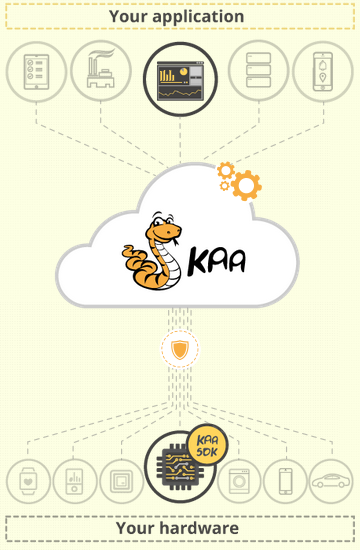
\includegraphics[scale=0.40]{../images/kaa/arqui.png}
		\caption{Arquitectura de KAA}
    \label{fig:kaalog}
	\end{center}
\end{figure}


\newpage

\subsection{Dispositivo receptor}

En éste aspecto no había muchas dudas en cuanto a las tecnologías a usar. Por una parte tenemos Raspbian, el sistema operativo oficial de Raspberry Pi basado en Debian. Usar algún otro sistema operativo ARM implicaría la incertidumbre sobre cualquier tipo de error en gran parte por el aspecto de los drivers.

\bigskip
Por otra parte tenemos el software desarrollado que se ejecuta en el dispositivo. Al igual que con el sistema operativo, el lenguaje de programación elegido desde un principio fue \textbf{Python} por su sencillez y número de bibliotecas. A medida que el desarrollo ha ido evolucionando Python ha demostrado ser el mejor candidato para el uso que se le pretendía dar, en gran parte gracias a la biblioteca \textbf{SoundDevice} que nos proporciona una manera realmente fácil de acceder y capturar datos de las interfaces de audio además de contar con numerosos ejemplos los cuales han sido de gran ayuda.

\bigskip
Por último, el dispositivo necesita hacer uso del SDK generado por KAA. Existen varias alternativas a la hora de generarlo y la más atractiva resultó ser \textbf{Java}. La interacción entre Python y Java se detallará más adelante.

\subsection{Almacenamiento de información}

Para almacenar datos de manera masiva existen varias alternativas como son Apache HBase, MongoDB, Apache Cassandra, Hive ó Redis. En éste aspecto la diferencia entre unas y otras es menores sin embargo hay una de ellas que destaca respecto a las otras por la facilidad de integración con KAA, es \textbf{Apache Cassandra} (\url{http://cassandra.apache.org/}).

\begin{figure}[!ht]
  \begin{center}
    
\includegraphics[scale=0.60]{../images/cassandra/logo.jpg}
    \label{fig:cassalog}
	\end{center}
\end{figure}

\begin{quote}\textit{ ''... is the right choice when you need scalability and high availability without compromising performance... Is best-in-class, providing lower latency for your users...''
}
\newline
\url{http://cassandra.apache.org/}
\end{quote}

Tras una breve documentación acerca de Cassandra se vió que era un software con unas características y una potencia a tener muy en cuenta además de su facilidad integración con KAA como se ha mencionado anteriormente, también se pueden definir funciones personalizadas en el lenguaje deseado y tiene una línea de comandos amigable. El lenguaje de consultas es CQL y su sintaxis no difiere mucho del resto de SGBD.


\subsection{Representación de información}

En éste apartado las opciones a tener en cuenta era Apache-Zeppelin y Jupyter. Ambas herramientas tienen el papel de representar la información que va a almacenar Cassandra. La integración entre la base de datos y Zeppelin se hace de una manera sencilla (ambas pertenecen a Apache) así como las consultas y visualización de datos, es por eso por lo que finalmente se optó por la opción de \textbf{Apache Zeppelin} (\url{https://zeppelin.apache.org/}).

\begin{figure}[!ht]
  \begin{center}
    
\includegraphics[scale=0.60]{../images/zeppelin/logo.png}
    \label{fig:zepplog}
	\end{center}
\end{figure}

\begin{quote}\textit{ ''A web-based notebook that enables interactive data analytics.
You can make beautiful data-driven, interactive and collaborative documents...''
}
\newline
\url{https://zeppelin.apache.org/}
\end{quote}

Apache Zeppelin nos va a permitir configurar una serie de Notebooks en forma de plataforma web en los que podremos realizar consultas a Cassandra para obtener los datos almacenados de los dispositivos receptores. Los datos se obtendrán mediante consultas CQL y podrán ser representados de varias formas, incluyendo distintos tipos de gráficos así como permitiendo la exportación de los mismos.

\newpage

\subsection{Plataforma Web de RSMap}

Para la plataforma web aunque las opciones eran varias en términos de lenguajes y frameworks. Finalmente la tecnología usada será Django que es un framework para aplicaciones web en Python.

\begin{figure}[!ht]
  \begin{center}
    
\includegraphics[scale=0.1]{../images/web/django-logo.png}
    \label{fig:drflog}
	\end{center}
\end{figure}

Las principales causas para la elección son la familiaridad con el mismo, que trabaja bajo el modelo Vista-Controlador, su documentación y el módulo Django-Rest-Framework que permite a los dispositivos comunicarse directamente con la web que será la encargada de representar en un mapa pequeños iconos que indiquen el paso de un vehículo.

El mapa es provisto por Google Maps.  Para ofrecer una navegación fluida concretamente en la sección del mapa se hará uso de jQuery y AJAX que nos sirven métodos para actualizar la información en el mismo mapa de manera automática y sin necesidad de recargar la página para ver los cambios.

El aspecto visual queda resuelto gracias a la librería Bootstrap (css) y una plantilla (html5) predefinida Open Source sobre la que efectuaremos las modificaciones necesarias para adaptarla a las necesidades de RSMap.

\section{Instalación y configuración de Raspberry Pi}

\subsection{Instalación}

En primer lugar se indica como instalar Raspbian en nuestra Raspberry Pi Jessie (basado en Debian), ésta ha sido la opción seleccionada como SO debido a que es el sistema oficial que provee Raspberry Pi.

\bigskip

El primer paso es descargarse la imagen de los servidores oficiales, la imagen usada se puede encontrar en \url{https://downloads.raspberrypi.org/raspbian/images/raspbian-2016-05-31/}

\begin{lstlisting}[language=bash,caption={Copia de Raspbian en tarjeta s y usb},label={lst:pi1}]
# muestra los discos del sistema
$ lsblk
# copia la imagen en el dispositivo /dev/sdb (tarjeta sd)
$ sudo dd bs=1M if=2016-05-27-raspbian-jessie.img of=/dev/sdb
# copia la particion del sistema en /dev/sdc (usb)
$ sudo dd bs=1M if=/dev/sdb2 of=/dev/sdc
\end{lstlisting}

\bigskip

Ahora editamos el archivo \textbf{/dev/sdb/boot/cmdline.txt} y añadimos la siguiente línea para que el sistema sólo use la tarjeta SD para arrancar y el dispositivo usb como disco del sistema, ésto aumentará la velocidad de lectura considerablemente:


\begin{lstlisting}[language=bash,caption={Modificando el dispositivo de arranque de Raspbian},label={lst:pi2}]
smsc95xx.turbo_mode=N dwc_otg.lpm_enable=0 console=ttyAMA0,115200 kgdboc=ttyAMA0,115200 console=tty1 root=/dev/sda1 rootfstype=ext4 elevator=noop rootwait # /dev/sda1 point to our USB drive
\end{lstlisting}

\bigskip

\subsection{Configuración}

Vamos a instalar el software necesario para interactuar con la tarjeta de sonio además de comprobar si el sistema la soporta y en caso afirmativo, establecerla como dispositivo de audio por defecto lo cual nos permitirá trabajar con ella después de cada reinicio ó apagado del dispositivo.

\begin{lstlisting}[language=bash,caption={Instalación del paquete alsa-utils},label={lst:pi3}]
$ sudo apt-get install alsa-utils
\end{lstlisting}

\begin{lstlisting}[language=bash,caption={Comprobano que el dispositivo es reconocido},label={lst:pi3}]
$ lsusb
Bus 001 Device 005: ID 0d8c:000c C-Media Electronics, Inc. Audio Adapter
Bus 001 Device 004: ID 0781:5567 SanDisk Corp. Cruzer Blade
Bus 001 Device 003: ID 0424:ec00 Standard Microsystems Corp. SMSC9512/9514 Fast Ethernet Adapter
Bus 001 Device 002: ID 0424:9514 Standard Microsystems Corp.
Bus 001 Device 001: ID 1d6b:0002 Linux Foundation 2.0 root hub
\end{lstlisting}

\begin{lstlisting}[language=bash,caption={Identificando los dispositivos de sonido disponibles en el sistema},label={lst:pi4}]
$ aplay -l
**** List of PLAYBACK Hardware Devices ****
card 0: ALSA [bcm2835 ALSA], device 0: bcm2835 ALSA [bcm2835 ALSA]
  Subdevices: 8/8
  Subdevice #0: subdevice #0
  Subdevice #1: subdevice #1
  Subdevice #2: subdevice #2
  Subdevice #3: subdevice #3
  Subdevice #4: subdevice #4
  Subdevice #5: subdevice #5
  Subdevice #6: subdevice #6
  Subdevice #7: subdevice #7
card 0: ALSA [bcm2835 ALSA], device 1: bcm2835 ALSA [bcm2835 IEC958/HDMI]
  Subdevices: 1/1
  Subdevice #0: subdevice #0
card 1: Set [C-Media USB Headphone Set], device 0: USB Audio [USB Audio]
  Subdevices: 1/1
  Subdevice #0: subdevice #0
	\end{lstlisting}

\bigskip

En éste caso el dispositivo se llama \textit{C-Media USB Headphone SetC-Media USB Headphone Set} cuyo identificador es 1, para establecerla como dispositivo de audio por defecto editamos \textit{/home/user/.asoundrc} con el siguiente contenido:


\begin{lstlisting}[language=bash,caption={Comprobano que el dispositivo es reconocido},label={lst:pi5}]
    pcm.!default {
      type hw
      card 1
  }

  ctl.!default {
      type hw
      card 1
  }
\end{lstlisting}

\section{Instalación y configuración de KAA}

\subsection{Instalación}

Para la instalación de KAA nos bastará con Amazon EC2, ya que el sistema de imágenes de SO contiene la versión más actual de KAA, los pasos a seguir son los siguientes:

Necesitamos una cuenta en Amazon EC2, tras registrarnos nos dirigimos al panel principal, y en el apartado \textit{INSTANCES} seleccionamos, \textit{Launch Instance} para crear una nueva máquina.

\begin{figure}[!ht]
  \begin{center}
    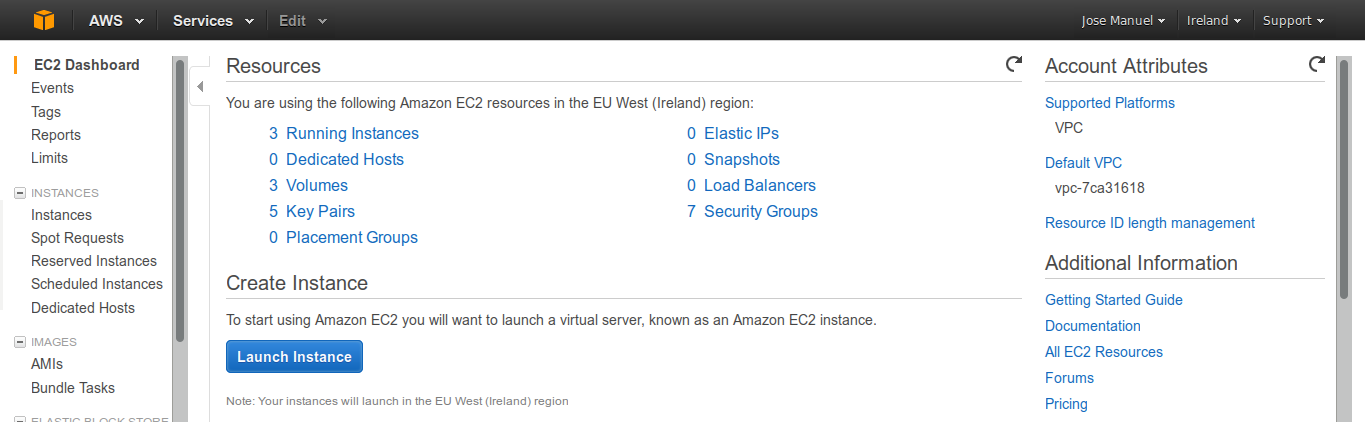
\includegraphics[scale=0.30]{../images/kaa/1.png}
		\caption{Dashboard de AmazonEC2}
    \label{fig:1}
	\end{center}
\end{figure}

\newpage

El segundo paso es dirigirse a \textit{Community AMIs} y en el cuadro de búsqueda escribimos \textit{kaa-sandbox}. Lo recomendable es usar la última versión, en éste caso se ha tomado la \textbf{versión 0.9}.

\begin{figure}[!ht]
  \begin{center}
    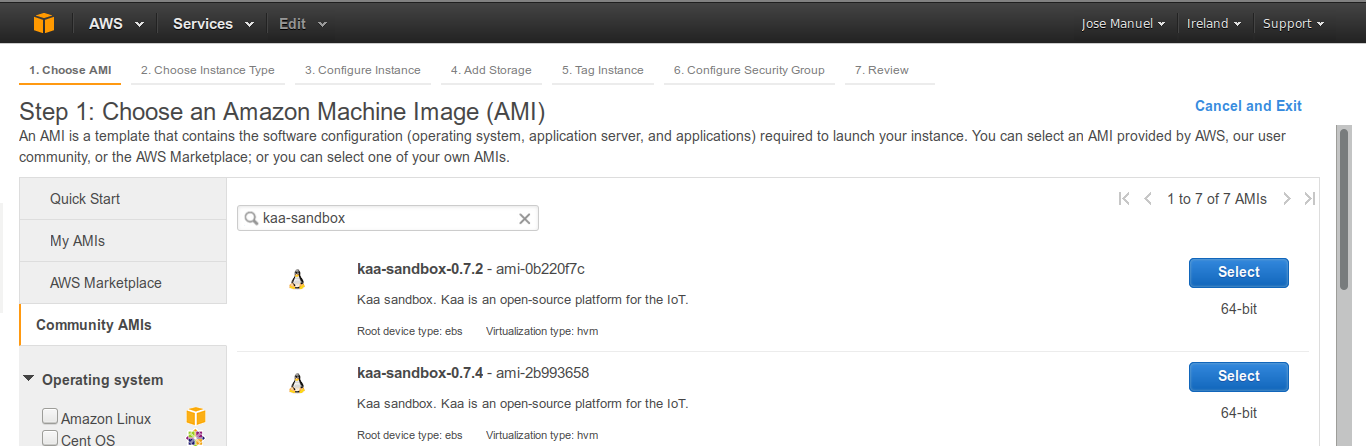
\includegraphics[scale=0.30]{../images/kaa/2.png}
		\caption{}
    \label{Instancias preconfiguradas de Kaa en EC2}
	\end{center}
\end{figure}

\newpage

Ahora debemos elegir el tipo de instancia, esto va directamente relacionado con la potencia de la misma. En un principio nos puede valer con las instancias de tipo \textit{free tier} y configurar la escalabilidad a medida de nuestras necesidades.

\begin{figure}[!ht]
  \begin{center}
    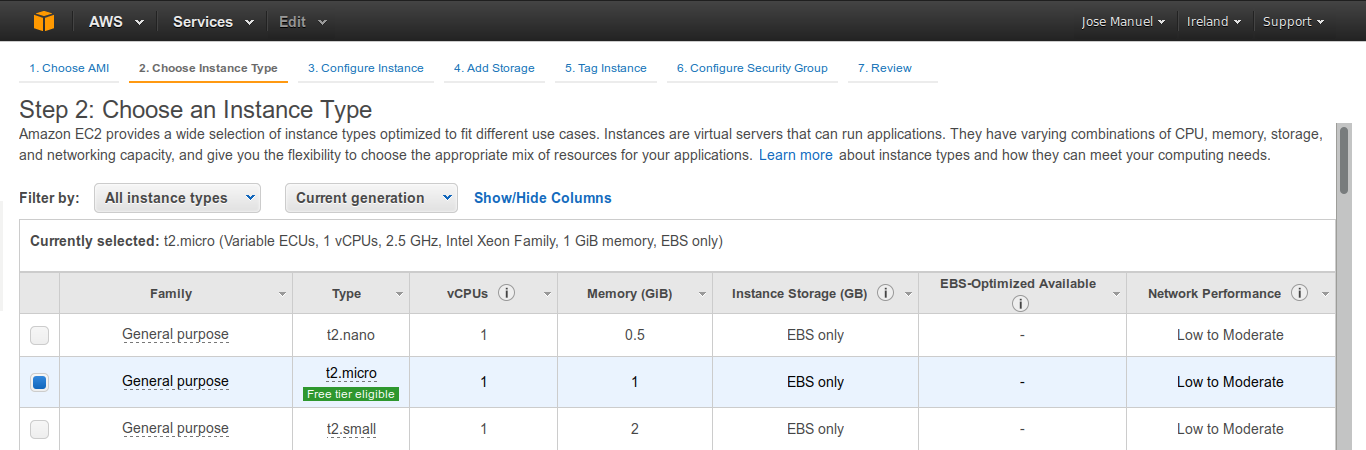
\includegraphics[scale=0.30]{../images/kaa/3.png}
		\caption{Selección del tipo de instancia}
    \label{fig:kaa}
	\end{center}
\end{figure}

En el siguiente paso podemos configurar algunas opciones relativas a la máquina, las que están por defecto son adecuadas por tanto no es necesario cambiar ninguna de ellas.

\begin{figure}[!ht]
  \begin{center}
    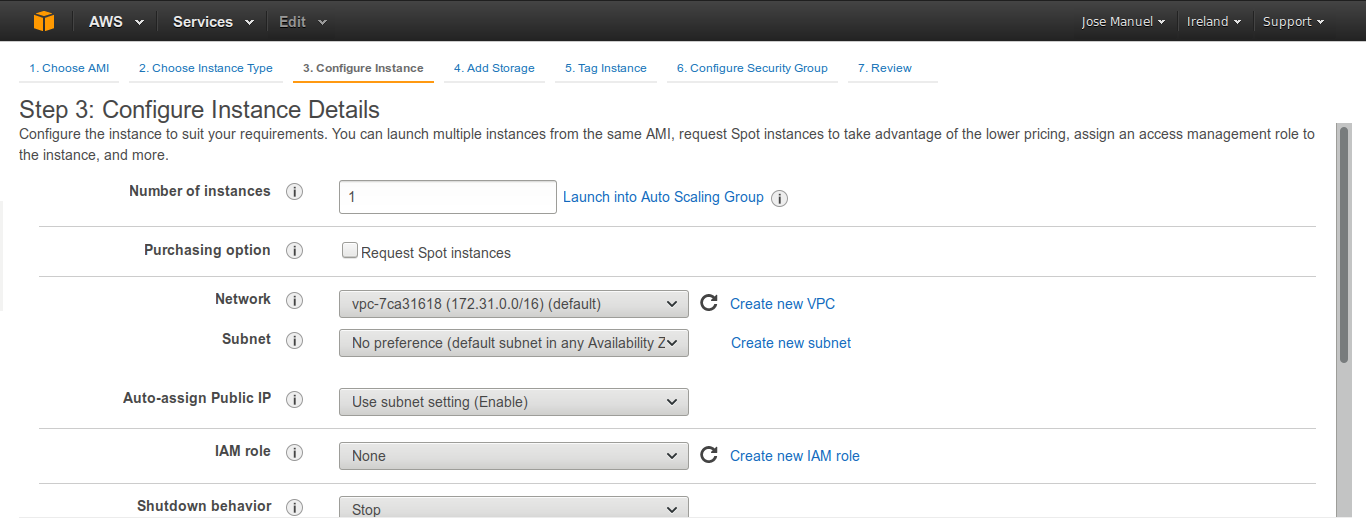
\includegraphics[scale=0.30]{../images/kaa/4.png}
		\caption{Configurar detalles de la instancia}
    \label{fig:kaa}
	\end{center}
\end{figure}

\newpage

El siguiente diálogo nos da la opción de configurar el almacenamiento, debido a que trabajamos en una instancia de tipo \textit{free tier} estamos restringidos a un tipo determinado de almacenamiento que al igual que el tipo de instancia, es suficiente por el momento.

\begin{figure}[!ht]
  \begin{center}
    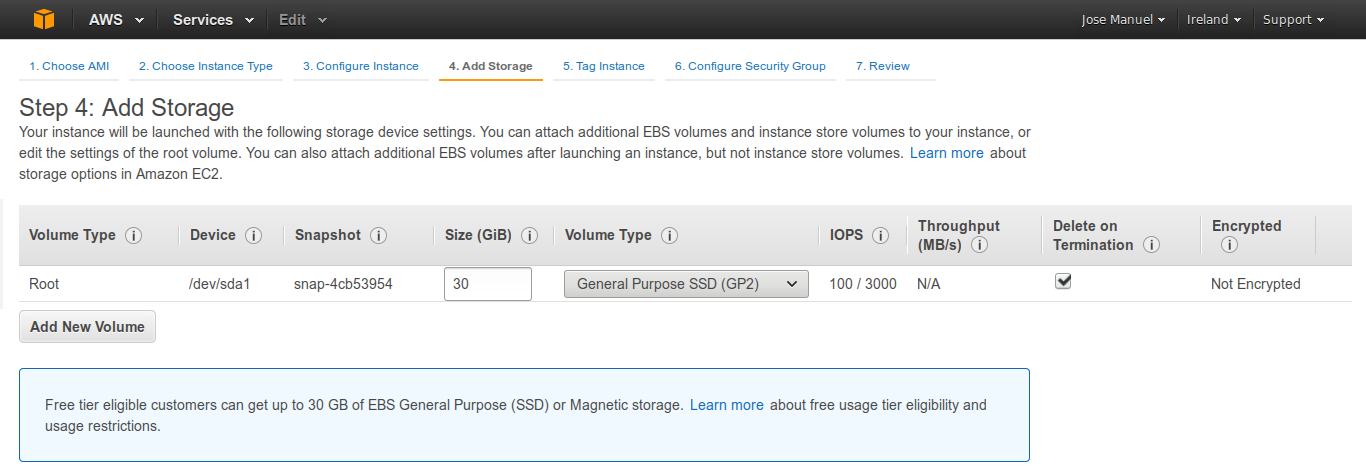
\includegraphics[scale=0.30]{../images/kaa/5.png}
		\caption{Selección de almacenamiento}
    \label{fig:kaa}
	\end{center}
\end{figure}

Los \textit{Security group} hacen referencia a la configuración de puertos, en la documentación de KAA se especifica cual debe ser, para el correcto funcionamiento y tiene una estructura como la de la \textit{ figura 6.7}.

\begin{figure}[!ht]
  \begin{center}
    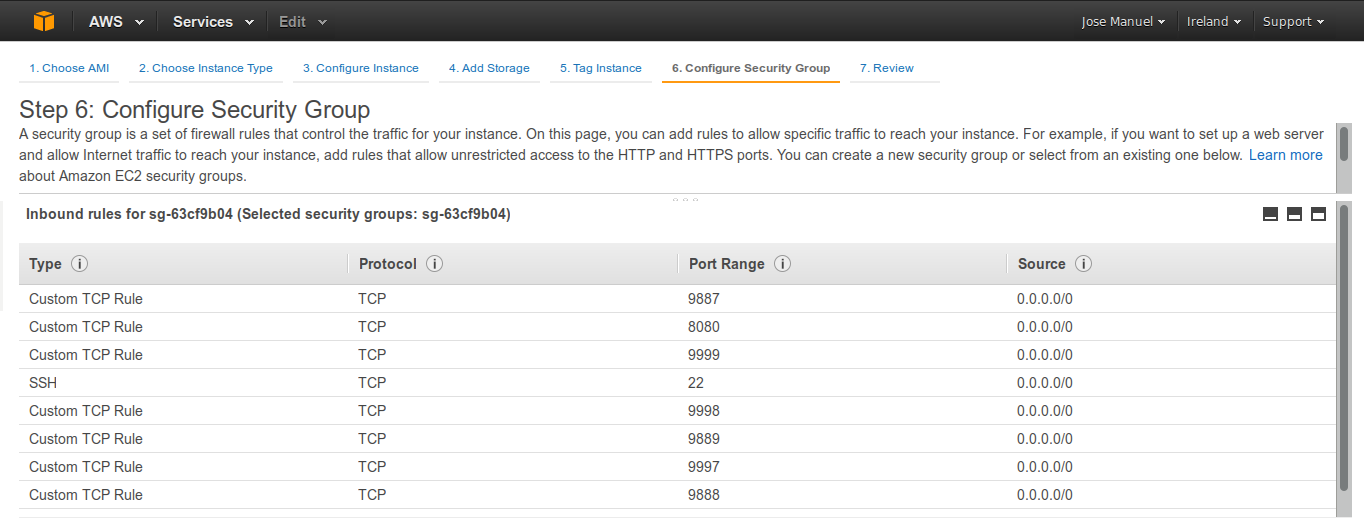
\includegraphics[scale=0.30]{../images/kaa/6.png}
		\caption{Configuración de puertos}
    \label{fig:kaa}
	\end{center}
\end{figure}

\newpage

Por último y no menos importante, debemos crear un par de llaves ó asignar uno existente. Ésto nos va a permitir conectarnos através de \textit{SSH} a la máquina en cualquier momento, si perdemos este par de claves perderemos el acceso a la máquina.

\begin{figure}[!ht]
  \begin{center}
    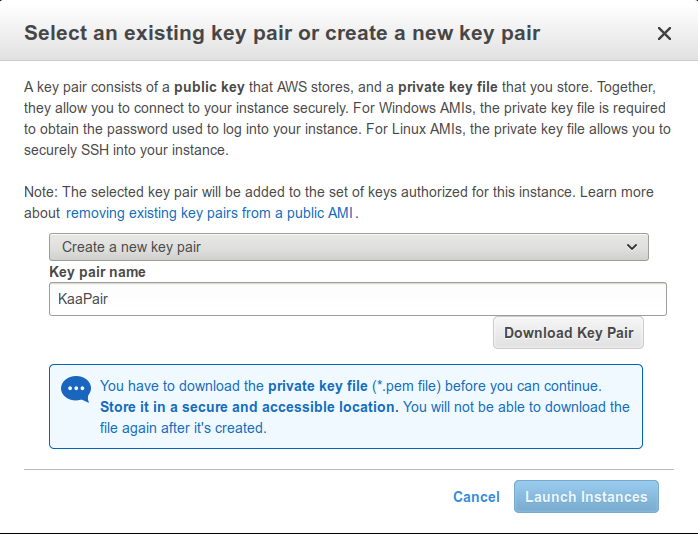
\includegraphics[scale=0.45]{../images/kaa/7.png}
		\caption{Creación de claves}
    \label{fig:kaa}
	\end{center}
\end{figure}

\subsection{Configuración}

Una vez tenemos el servicio instalado la configuración es trivial debido a que KAA provee un servicio web através del que definimos todo lo necesario.

Antes de empezar merece la pena destacar que existe 3 tipos de usuarios en KAA:

\begin{itemize}
	\item \textbf{Admin: } puede dar de alta Tenant admins.
	\item \textbf{Tenant admin: } puede dar de alta aplicaciones y Tenant developers.
	\item \textbf{Tenant developer:} puede configurar las aplicaciones y generar SDK's.
\end{itemize}

\bigskip

El primer paso es establecer la ip pública de KAA, accediendo desde el menú \textit{management}.

\begin{figure}[!ht]
  \begin{center}
    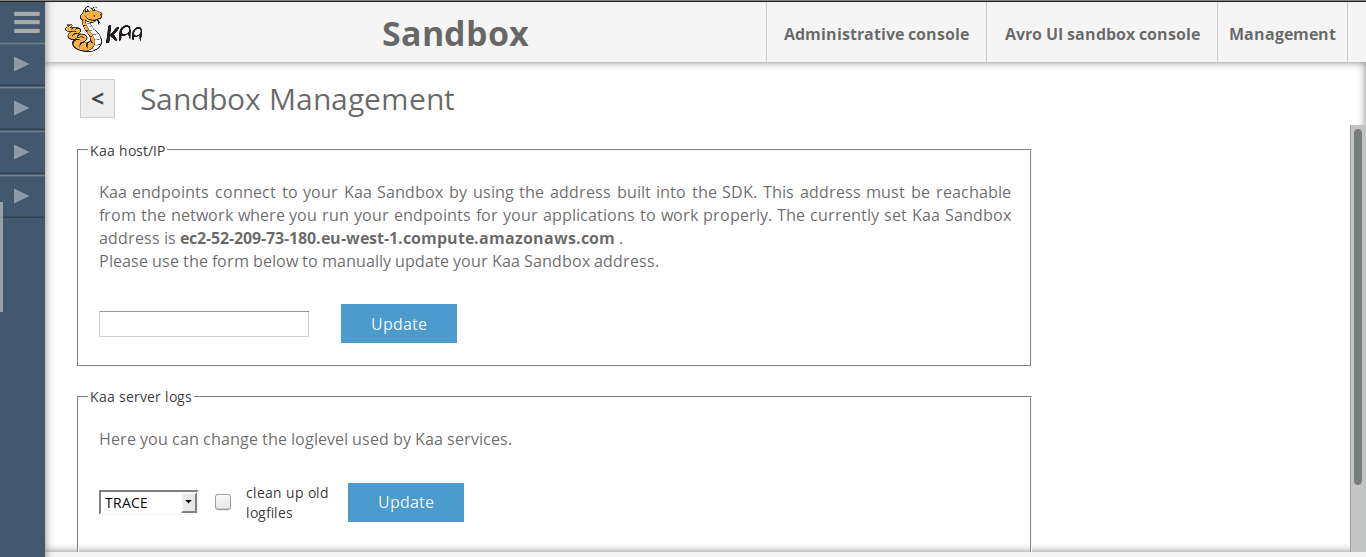
\includegraphics[scale=0.30]{../images/kaa/8.png}
		\caption{Sección Management}
    \label{fig:kaa}
	\end{center}
\end{figure}

\newpage

Ahora nos dirigimos a \textit{Administrative console} y nos logeamos como Tenant admin para dar de alta una nueva aplicación.

El tipo de credencial seleccionado será \textit{Trusful} de esta forma permitiremos a cualquier cliente conectarse a nuestra aplicación sin necesidad de autentificarse.

\begin{figure}[!ht]
  \begin{center}
    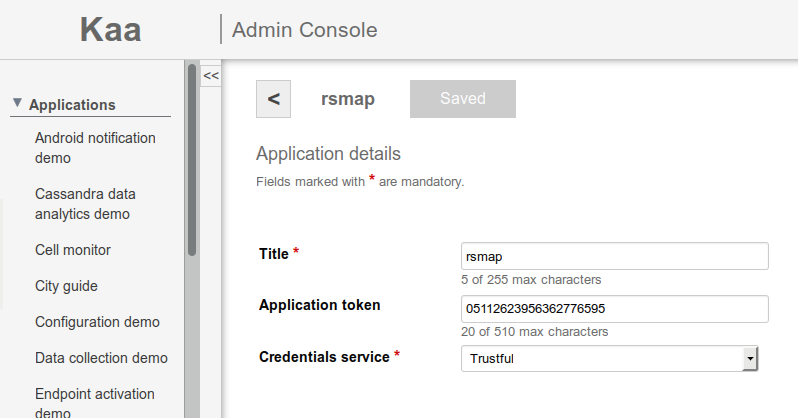
\includegraphics[scale=0.50]{../images/kaa/11.png}
		\caption{Creación de la nueva aplicación}
    \label{fig:kaa}
	\end{center}
\end{figure}

Nos logeamos con una cuenta Tenant Developer, vamos a proceder a crear la estructura de datos que define los campos y el tipo de los mismos que pertenecerán a nuestra aplicación.

Éste paso puede hacerse desde la interfaz web o subiendo un archivo \textit{json}. En nuestro caso vamos a valernos del \textit{json} por comodidad.

\begin{figure}[!ht]
  \begin{center}
    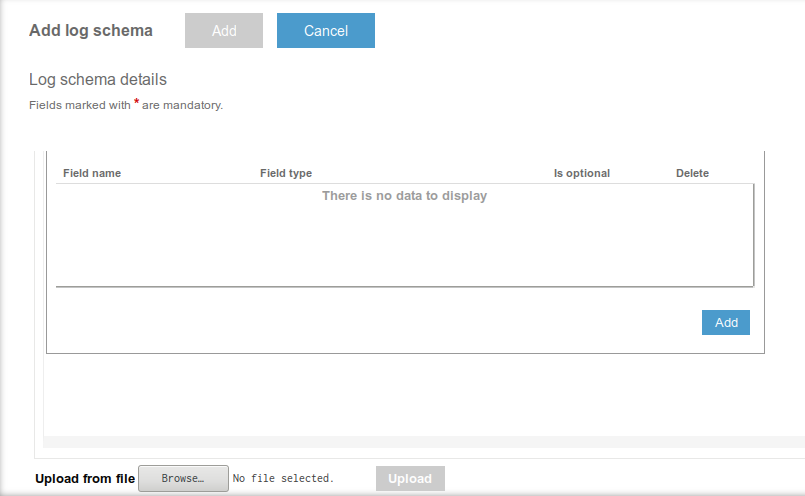
\includegraphics[scale=0.45]{../images/kaa/11-2.png}
		\caption{Definiendo esquemas de datos}
    \label{fig:kaa}
	\end{center}
\end{figure}

\newpage

Aquí se definen los campos que KAA va a proveer en el SDK generado, lo que se traduce en que éste mismo SDK nos ofrecerá una clase con los campos definidos en éste apartado. El campo \textit{namespace} indica en que paquete se encontrará la clase correspondiente al esquema definido dentro del SDK generado. KAA hace uso de Apache Avro para definir esquemas de serialización de datos. Ésto le permite manejar internamente la información almacenada en los esquemas.

\bigskip

\begin{lstlisting}[language=json,caption={Esquema de datos en JSON},label={lst:json_personal}]
{
	"type" : "record",
	"name" : "AudioReport",
	"namespace" : "org.kaaproject.kaa.schema.rsmap",
	"fields" : [ {
		"name" : "timestamp",
		"type" : "long"
	}, {
		"name" : "zoneId",
		"type" : {
			"type" : "string",
			"avro.java.string" : "String"
		}
	}, {
		"name" : "deviceId",
		"type" : {
			"type" : "string",
			"avro.java.string" : "String"
		}
	}, {
		"name" : "level",
		"type" : "double"
	} ]
}
\end{lstlisting}

Ahora ya tenemos el esquema definido en KAA como muestran la \textit{figura 6.12} y la \textit{figura 6.13}:

\begin{figure}[!ht]
  \begin{center}
    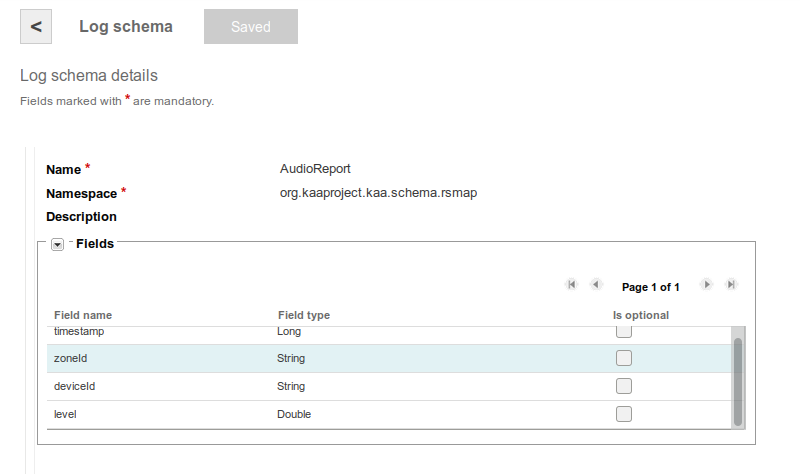
\includegraphics[scale=0.45]{../images/kaa/13.png}
		\caption{Esquema de datos definido 1}
    \label{fig:kaa}
	\end{center}
\end{figure}

\begin{figure}[!ht]
  \begin{center}
    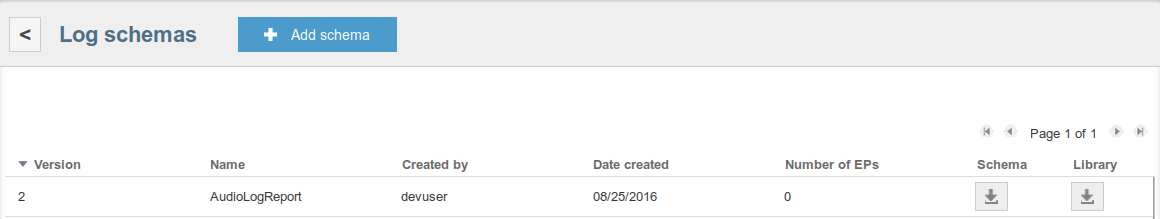
\includegraphics[scale=0.30]{../images/kaa/14.png}
		\caption{Esquema de datos definido 2}
    \label{fig:kaa}
	\end{center}
\end{figure}

\newpage

\newpage
\newpage
\newpage

\section{Instalación y configuración de Apache Cassandra.}

\subsection{Instalación}

El proceso para definir la máquina virtual que contiene Cassandra es el mismo que el de KAA a excepción de dos puntos, el primero es el tipo de instancia. Dentro de \textit{Community AMIs} debemos buscar \texit{Cassandra} y elegir la versión más reciente.

\begin{figure}[!ht]
  \begin{center}
    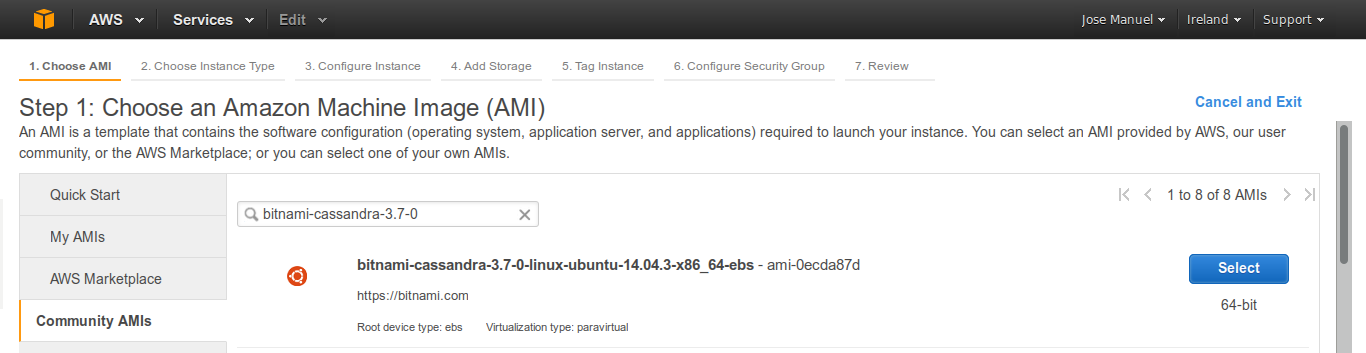
\includegraphics[scale=0.30]{../images/cassandra/1.png}
		\caption{Imagen de Cassandra en EC2}
    \label{fig:kaa}
	\end{center}
\end{figure}

El otro punto que difiere es el \textit{Security Group}, dado que los puertos que necesitamos son distintos la configuración debe quedar tal que así:

\begin{figure}[!ht]
  \begin{center}
    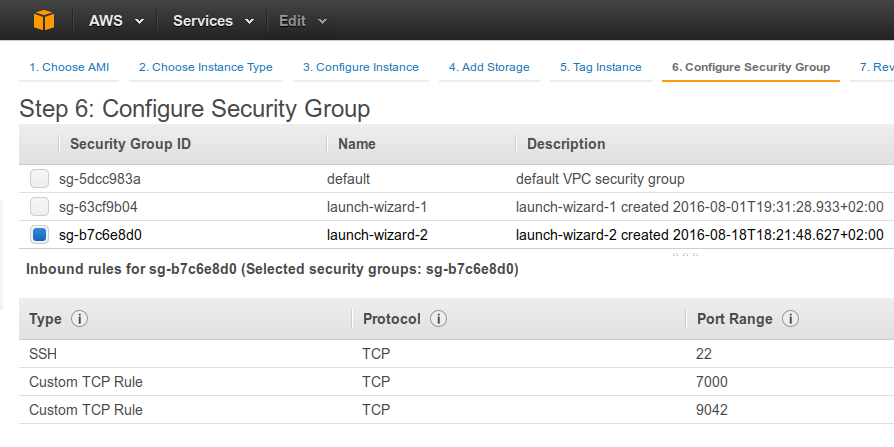
\includegraphics[scale=0.30]{../images/cassandra/2.png}
		\caption{Security Group para Cassandra}
    \label{fig:kaa}
	\end{center}
\end{figure}

\newpage

\subsection{Configuración}

Para comprobar que funciona correctamente accedemos mediante \textit{SSH} y nos logeamos en la shell de Cassandra haciendo uso del comando \textbf{cqlsh} como indica la \textit{figura 6.16}.

\begin{figure}[!ht]
  \begin{center}
    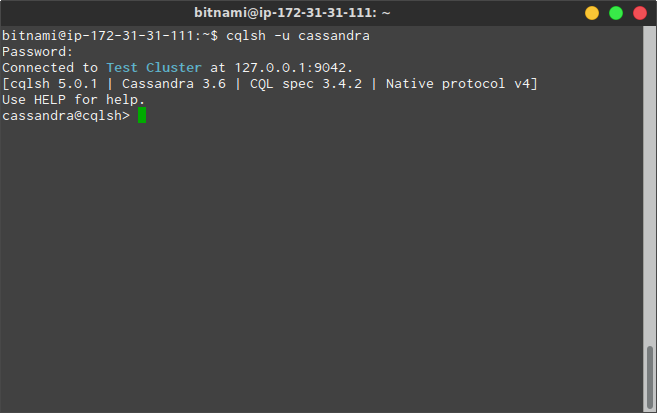
\includegraphics[scale=0.55]{../images/cassandra/3.png}
		\caption{Accediendo al servidor de Cassandra}
    \label{fig:kaa}
	\end{center}
\end{figure}

\newpage

Vamos a crear un \textit{Keyspace} que contendrá las tablas de nuestra aplicación, para ello usamos la siguiente sentencia:

\begin{lstlisting}[language=json,caption={Keyspace en Cassandra},label={lst:json_personal}]

CREATE KEYSPACE rsmapv0 WITH replication = {
	'class': 'SimpleStrategy',
	'replication_factor': 1
};

\end{lstlisting}

\textit{SingleStrategy} indica que sólo usaremos un \textit{Datacenter} y en \textit{replication factor} se indica el número de nodos de copia que queremos establecer.

\newpage

Ahora es momento de volver a KAA y definir el \textit{LogAppender} que se encargará de decirle a los clientes cómo y donde tienen que enviar los datos mediante el SDK. En nuestro caso será la base de datos que acabamos de configurar. Ésto lo haremos en la sección de Log appenders mediante un fichero \textit{json} con la siguiente estructura:


\begin{lstlisting}[language=json,caption={Esquema de log appender en JSON},label={lst:json_personal}]

{
   "cassandraServers":[
      {
         "host":"ec2-52-210-20-84.eu-west-1.compute.amazonaws.com",
         "port":9042
      }
   ],
   "cassandraCredential":{
      "org.kaaproject.kaa.server.appenders.cassandra.config.gen.CassandraCredential":{
         "user":"####",
         "password":"####"
      }
   },
   "keySpace":"rsmapv0",
   "tableNamePattern":"rows",
   "columnMapping":[
      {
         "type":"EVENT_FIELD",
         "value":{
            "string":"zoneId"
         },
         "columnName":"zone_Id",
         "columnType":"TEXT",
         "partitionKey":true,
         "clusteringKey":false
      },
      {
         "type":"EVENT_FIELD",
         "value":{
            "string":"timestamp"
         },
         "columnName":"timestamp",
         "columnType":"BIGINT",
         "partitionKey":false,
         "clusteringKey":true
      },
      {
         "type":"EVENT_FIELD",
         "value":{
            "string":"deviceId"
         },
         "columnName":"device_Id",
         "columnType":"TEXT",
         "partitionKey":false,
         "clusteringKey":true
      },
      {
         "type":"EVENT_FIELD",
         "value":{
            "string":"level"
         },
         "columnName":"level",
         "columnType":"DOUBLE",
         "partitionKey":false,
         "clusteringKey":false
      }
   ],
   "clusteringMapping":[
      {
         "columnName":"timestamp",
         "order":"DESC"
      }
   ],
   "cassandraBatchType":{
      "org.kaaproject.kaa.server.appenders.cassandra.config.gen.CassandraBatchType":"UNLOGGED"
   },
   "cassandraSocketOption":null,
   "executorThreadPoolSize":1,
   "callbackThreadPoolSize":2,
   "dataTTL":0,
   "cassandraWriteConsistencyLevel":{
      "org.kaaproject.kaa.server.appenders.cassandra.config.gen.CassandraWriteConsistencyLevel":"ONE"
   },
   "cassandraCompression":{
      "org.kaaproject.kaa.server.appenders.cassandra.config.gen.CassandraCompression":"NONE"
   },
   "cassandraExecuteRequestType":{
      "org.kaaproject.kaa.server.appenders.cassandra.config.gen.CassandraExecuteRequestType":"SYNC"
   },
   "minLogSchemaVersion":1,
   "maxLogSchemaVersion":2147483647,
   "pluginTypeName":"Cassandra",
   "pluginClassName":"org.kaaproject.kaa.server.appenders.cassandra.appender.CassandraLogAppender",
   "headerStructure":[

   ]
}

\end{lstlisting}

Los campos a tener en consideración en este archivo son los siguientes:

\begin{itemize}
	\item \textbf{Host:} hace referencia a la IP de Cassandra.
	\item \textbf{Port:} puerto de Cassandra.
	\item \textbf{User:} usuario de Cassandra.
	\item \textbf{Password:} contraseña de Cassandra.
	\item \textbf{keySpace:} keySpace de Cassandra.
	\item \textbf{tableNamePattern:} nombre de la tabla a crear.
	\item \textbf{columnMapping:} equivalencia entre los campos definidos en el esquema y las columnas que contendrá cada entrada en la base de datos.
\end{itemize}


Por tanto en éste fichero se especifica el usuario y la contraseña de Cassandra que han sido ocultados por seguridad, la IP pública del servidor Cassandra y campos del final indican la equivalencia entre los campos de esquema creado anteriormente y las tablas en Cassandra.

Una vez generemos el esquema, KAA se conectará a Cassandra y creará las tablas según el formato que le hemos indicado en el mapa \textit{columnMapping}.

\bigskip

Un factor importante es el diseño de las tablas, pues las consultas en Cassandra son dependientes de la estructura de la base de datos. El tipo de campos que determinan la estructura de la tabla son los siguientes:

\begin{itemize}
\item \textbf{partitionKey, } que es la responsable de la distribución de los datos entre los nodos de Cassandra.
\item \textbf{clusteringKey, } que se usa para ordenar los elementos dentro de una partición.
\end{itemize}

En el caso de RSMap se usa el campo \textit{zoneId} como \textit{partition key} y \textit{timestamp y deviceId} como \textit{clustering key} lo que nos garantiza que podremos hacer consultas del tipo:


\begin{lstlisting}[language=cql,caption={Mécanica de consultas en CQL según la estructura de tablas},label={lst:json_personal}]

SELECT * FROM abc WHERE partitionKey = 'X';
SELECT * FROM table WHERE partitionKey = 'X' AND clusteringKey  = 'Y';

\end{lstlisting}

\bigskip

Tras guardar el \textit{log appender} podemos comprobar como se ha creao la tabla \textit{rows} dentro del keyspace \textit{rsmapv0}. Para realizar ésta comprobación accedemos a la shell de Cassandra como muestra la \textit{figura 6.17	}.

\begin{figure}[!ht]
  \begin{center}
    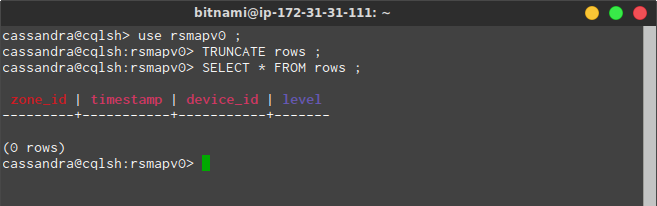
\includegraphics[scale=0.65]{../images/cassandra/4.png}
		\caption{Comprobación de las tablas creadas}
    \label{fig:kaa}
	\end{center}
\end{figure}

\newpage

Cuando la tabla contiene datos la consulta se muestra así:

\begin{figure}[!ht]
  \begin{center}
    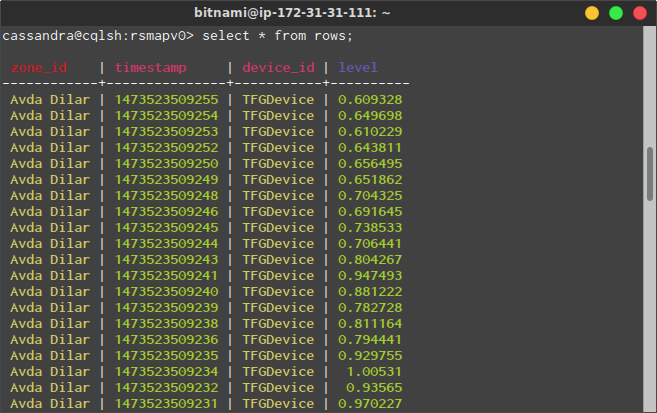
\includegraphics[scale=0.65]{../images/cassandra/6.png}
		\caption{Cassandra con datos almacenados}
    \label{fig:kaa}
	\end{center}
\end{figure}

Para finalizar vamos a crear dos funciones en java dentro del Keyspace que nos ayudarán a visualizar y consultar los datos posteriormente. La necesidad de definir estas funciones viene dada porque el campo TimeStamp se almacena bajo el formato UnixTimestamp que nosproporciona los milisegundos actuales transcurridos desde 1970. Es importante destacar que estas funciones pueden ser definidas en el lenguaje que queramos, en nuestro caso vamos a usar Java.

\bigskip

La primera convierte un \textit{timestamp} en una hora legible, las otras dos nos ayudarán a seleccionar los datos de un minuto atrás hasta la fecha actual y de una hora atrás hasta la fecha actual.

\begin{figure}[!ht]
  \begin{center}
    \includegraphics[scale=0.65]{../images/cassandra/5.png}
		\caption{Funciones dentro de Cassandra}
    \label{fig:kaa}
	\end{center}
\end{figure}

\newpage

Si queremos hacer uso de éstas funciones debemos editar el fichero \textbf{/home/bitnami/stack/cassandra/conf} y cambiar la línea:

enable user defined functions: false

por:

enable user defined functions: true

\bigskip

Ya sólo nos queda reiniciar el servicio:

\begin{lstlisting}[language=bash,caption={Reiniciando Cassandra},label={lst:rcas}]
	$ sudo ./stack/ctlscript.sh stop cassandra
	$ sudo ./stack/ctlscript.sh start cassandra
\end{lstlisting}

A modo de resumen, hasta el momento tenemos la plataforma KAA desplegada, en ella se encuentra el esquema de datos a usar y el LogAppender que indica a donde se van a remitir los datos. Además tenemos Apache Cassandra desplegado y con las tablas necesarias creadas para empezar a enviar información de las señales detectadas. Ésto quiere decir estamos en disposición de generar el SDK que usarán los clientes para connectarse a Cassandra.

\bigskip

Para generar el SDK accedemos a la interfaz web de KAA. Los SDK's se generan bajo un sistema de versiones lo que nos posibilita tener varios para una misma aplicación con distinto funcionamiento. El control de éstas versiones se gestiona mediante perfiles SDK por lo que si queremos obtener el nuestro debemos definir en primer lugar un perfil en el que también se deben especificar las versiones para los esquemas y log appenders.

Una vez nos encontremos en la interfaz buscamos la aplicación creada que se detalló en la sección de \textit{Configuración de KAA} y nos situamos en la opción \textit{SDK profiles} / \textit{Add SDK Profile}.


\begin{figure}[!ht]
  \begin{center}
    \includegraphics[scale=0.30]{../images/sdk/1.png}
		\caption{Definición del SDK}
    \label{fig:kaa}
	\end{center}
\end{figure}

\newpage

Por último pulsamos la opción \textit{Generate SDK} la cual nos muestra una ventana en la que debemos escoger sobre qué lenguaje se generará el SDK. RSMap usa el SDK generado en Java.


\begin{figure}[!ht]
  \begin{center}
    \includegraphics[scale=0.30]{../images/sdk/2.png}
		\caption{Definición del SDK}
    \label{fig:kaa}
	\end{center}
\end{figure}

\newpage

\section{Desarrollo del módulo de detección de vehículos.}

El código completo de éste módulo se encuentra en el repositorio \url{https://github.com/RSMap/RSMapPi}, dentro de la organización \url{https://github.com/RSMap} que alberga el proyecto RSMap completo.

\bigskip

Para analizar la estructura podemos hacer una clara división en dos partes, por un lado tenemos el módulo en python que se encarga de interactuar con la tarjeta de sonido, tomar los datos y enviarlos. La segunda parte es el módulo en java que se encarga de usar el SDK generado en KAA para enviarlos a Cassandra.

\subsection{Módulo de detección}

Para detallarlo de una manera clara se analizarán fragmentos de código separadamente, aunque todos ellos pertenecen al mismo archivo \textit{(RSMapPi/\/analyzer/\/VehicleDetection.py)} pero antes a modo de resumen se enumeran las librerías más reseñables y la secuencia que sigue el programa a lo largo de su ejecución.

\subsubsection{Dependencias}

Las dependencias externas y necesarias de éste módulo se encuentran especificadas en el archivo \textit{(RSMapPi/\/analyzer/\/requirements.txt)}. Las más importantes son:

\begin{itemize}
	\item \textbf{sounddevice==0.3.4:} es la más importante ya que mediante ella se accede al dispositivo para capturar los datos. Hay que destacar que los ejemplos de su documentación han sido de gran ayuda a la hora del desarrollo de éste módulo.
	\item \textbf{numpy==1.11.1:} es la librería por excelencia para el análisis científico de datos en Python.
	\item \textbf{requests==2.11.1:} nos proporciona una cómoda interfaz para efectuar peticiones HTTP que serán usadas para interactuar con la API Rest.
\end{itemize}

\newpage

Además se han usado algunas otras dependencias pertenecientes a python, su instalación no es necesaria pues vienen con el compilador del lenguaje, ellas son:

\begin{itemize}
	\item \textbf{queue:} contine la estuctura de datos de cola, sobre la que se insertaran y leerán los datos obtenidos.
	\item \textbf{threading:} nos permite crear hebras y procesos.
	\item \textbf{socket:} nos servirá para enviar los datos obtenidos desde Python al SDK de KAA que, recordemos que está en Java.
\end{itemize}

\bigskip

\subsubsection{Resumen de ejecución}

\bigskip

En primer lugar se realiza una petición a la API para dar de alta el dispositivo en la lista de los receptores que se encuentran enviando datos. Si esa petición nos devuelve el código 400 significa que ese dispositivo ya se encuentra dado de alta, por lo que en ese caso vamos a realizar otra petición, ésta vez sobre la ruta asignada a ese dispositivo en concreto para indicar que el dispositivo se ha conectado y empezará a retransmitir datos en breve. En caso de que el dispositivo no exista, se da de alta con el payload que contiene toda la información asociada a el.

\bigskip

Una vez el dispositivo se identifica mediante la API, se abre un socket sobre el mismo equipo (localhost), éste servirá para enviar los datos obtenidos desde Python a Java. Los dos primeros mensajes que se envían son la cadena de localización del dispositivo y su identificador.

\bigskip

A continuación se definen una serie de variables que serán usadas para la detección y análisis del tráfico.
Tras ésto se lanzan dos hebras, una trabajará con la función \textit{producer} y la otra con la función \textit{consumer}.

\bigksip

La hebra \textit{producer} hace uso de la librería \textbf{Sound device} a la que llama con los parámetros definidos anteriormente, el más destacable es callback, que hace referencia a la función \textit{callback} la cual tiene el cometido generar los bloques con los datos numéricos extraidos desde la tarjeta de sonido y ponerlos en la cola.
\bigskip

La hebra \textit{consumer} es la encargada de analizar la información puesta en la cola y enviar las señales tanto al SDK (valores que se almacenarán) como a la API Rest (valores que se representarán en el mapa). Cuando el programa recibe una señal de interrupción (\textit{enter, 'q' o 'Q'}) el productor pondrá en la cola un objeto de llamado \textit{\_sentinel} el cual le indicará al consumidor que el programa va a finalizar. El consumidor envía las señales de parada a la API Rest, que borrará el dispositivo de la lista de dispositivos retransmitiendo así como al programa en Java que cerrará la conexión con Cassandra.

\newpage
\subsubsection{Código}

Al comienzo del fichero se definen una serie de variables que serán usadas cuando el dispositivo envíe información. Gracias a ellas éste quedará identificado por un id (\textit{device\_id}), una localización en formato texto (\textit{device\_location}) y una localización geográfica (\textit{latitude y longitude}).

A continuación se generan los payloads iniciales que se usarán para realizar las peticiones sobre la API, éstos tiene estructura de map \{'clave' : valor\} y tenemos dos tipos:

\begin{itemize}
	\item \textbf{new\_device\_payload:}

	contiene toda la información asociada al dispositivo, es usado cuando el dispositivo no está registrado en la plataforma web.
	\item \textbf{existing\_device\_payload:}

	contiene únicamente el nivel iniciado a -1, ésto permitira identificarlo como nuevo dispositivo y representarlo en el mapa con un icono que indique una nueva conexión.
\end{itemize}

En la parte final de éste bloque se definen las URLS que se necesitarán para comprobar el estado del dispositivo en el sistema.

\begin{itemize}
	\item \textbf{signals\_list\_url: }

	referencia a la url que contiene todos los dispositivos registrados.
	\item \textbf{signal\_url: }

	referencia a la url que identifica un dispositivo en concreto.
\end{itemize}

\begin{lstlisting}[language=python,caption={Parámetros usados para la comunicación con la API},label={lst:pi1}]
	# device id (case sensitive)
	device_id = 'TFGDevice'
	# device location (name)
	device_location = 'Avda Dilar'
	# device coordinates
	latitude = '37.177336'
	longitude = '-3.598557'
	# signal_type (default unknown)
	signal_type = 'u'
	# level -1 means device is connected and it will send data soon.
	level = '-1.0'
	# new_device_payload contains all related info with a map structure
	new_device_payload = {'device_id':device_id, 'lat':latitude, 'long':longitude, 'level':level, 'type':signal_type}
	# if device exists, only level is needed
	existing_device_payload = {'level': level}
	# rest urls
	signals_list_url = 'http://52.210.3.41/api/signals/'
	signal_url = 'http://52.210.3.41/api/signal/'+device_id+'/'
\end{lstlisting}

El siguiente bloque se encarga de hacer uso de las URL's y Payloads definidos anteriormente

\begin{lstlisting}[language=python,caption={Identificación de dispositivo mediante la API},label={lst:pi1}]
# rest first request
req = requests.post(signals_list_url, new_device_payload)

# check rest response
if(req.status_code == 400):
    print("Device already exists, sending connect signal")
    req = requests.patch(signal_url, existing_device_payload)
    if(req.status_code == 200):
        print("Connection successful")
    else:
        print("Can't send connected signal, exiting")
        sys.exit()
elif(req.status_code == 201):
    print("Connection successful, device added to device's database")
else:
    print("Device can't connect to rest service, check your connection.")
    sys.exit()
\end{lstlisting}

Cuando realizamos una petición HTTP obtenemos un valor numérico que nos indica el resultado de dicha petición. En base a los códigos obtenidos podemos saber si el dispositivo se encontraba dado de alta, por lo que no se puede sobreescribir con una petición POST (\textit{código 400}) o por el contrario si se añadió satisfactoriamente (\textit{código 201}).

En el caso de no poder realizar la petición POST usamos la petición PATCH que básicamente es un \textit{update} sobre el objeto en Django que contiene la información del dispositivo, es aquí donde se usa la URL definida en la variable \textit{signal\_url} que hace referencia directa al dispositivo en cuestión.

En cualquier caso, el campo \textit{level} será establecido a -1, lo que sobre el mapa se traducirá en el icono de conexión.

\newpage

El siguiente paso es conectarse al Socket creado por \textit{DataSender.java} que deberá estar lanzado y esperando conexiones.

\begin{lstlisting}[language=python,caption={Conexión con Java mediante un Socket},label={lst:pi1}]
	# Connecting to DataSender socket on localhost
	socket = socket.socket()
	socket.connect(('localhost', 5000))
	# Send device location
	device_location_sock = device_location+"\n"
	device_location_bytes = bytes(device_location_sock, 'utf-8')
	socket.send(device_location_bytes)
	# Send device id
	device_id_sock = device_id+"\n"
	device_id_bytes = bytes(device_id_sock, 'utf-8')
	socket.send(device_id_bytes)
\end{lstlisting}

Se le envían dos mensajes iniciales que contienen la cadena de localización y el id del dispositivo los cuales serán usados a posteriori por \textit{DataSender.java} para añadirlos a Cassandra. No se puede pasar una cadena como tal, es por eso por lo que se convierten en Bytes antes de enviarlos.

\bigskip

Ahora se definen las variables necesarias para la captura e identificación de vehículos.

\begin{lstlisting}[language=python,caption={Variables corresopndientes al análisis},label={lst:pi1}]
 # multiplier factor
 gain = 10
  # number of cuantization levels
 levels = 100
 # system device id
 device = 2
 # block time (ms)
 block_duration = 100
 # sample rate
 samplerate = 44100
 # high sample rate
 high = 2000
 # low sample rate
 low = 450
 # cuantization value
 delta_f = (high - low) / levels
 # window will divided in bands, fftsize defines the resolution on freq domain
 fftsize = np.ceil(samplerate / delta_f).astype(int)
 # window freq resolution
 low_bin = np.floor(low / delta_f)
 # vehicle threshold
 threshold = 0.59
 # consequtive blocks, its may depend of the road conditions
 consequtive_blocks = 50
\end{lstlisting}

Las variables \texit{threshold} y \texit{consequtive\_blocks} tienen relación directa con la identificación de vehículos. La primera indica el umbral mínimo que deben tener los valores obtenidos por cada bloque obtenido mientras que la segunda indica qué número de bloques necesitamos por encima de ese umbral para considerar que un vehículo ha pasado.

El resto poseen la misma estructura que las del ejemplo que proporciona la librería \textit{SoundDevice} para cuantizar los valores obtenidos através de una entrada de audio. ( \url{http://python-sounddevice.readthedocs.io/en/0.3.4/examples.html#real-time-text-mode-spectrogram} )


\bigskip

La esencia de la hebra productora es la llamada a \textbf{InputStream} que abre un canal de comunicación con la tarjeta de sonido. Toma como argumentos los valores definidos anteriormente y una función llamada \textit{callback}, que es la encargada de generar cada bloque y ponerlo en la cola. Cada bloque consta de una serie de valores que tras aplicarle la Transformada Rápida de Fourier son sumados obtenieno así el valor global para cada bloque.

\begin{lstlisting}[language=python,caption={Hebra productora},label={lst:pi1}]
with sd.InputStream(
	device=device,
	channels=1,
	callback=callback,
	blocksize=int(samplerate * block_duration / 1000),
	samplerate=samplerate
)
\end{lstlisting}

\bigskip

El código perteneciente a la hebra consumidora consiste en un bloque que se ejecuta mientras no obtenga una señal de parada, en tal caso se envía una señal de desconexión a la API usando el método DELETE que eliminará el modelo asociado al dispositivo en Django y otra a \textit{DataSender.java}. El código encargado de filtrar los datos es el siguiente:

\begin{lstlisting}[language=python,caption={Hebra consumidora},label={lst:pi1}]
if(data > threshold ):
	# global block consequtive count
	consequtive += 1
	local_consequtive += 1
	local_data_sum += data
	if(local_consequtive == consequtive_blocks):
		# if detected > consequtive_blocks send to api rest
		existing_device_payload = {
			'level': str(local_data_sum)
		}
		req = requests.patch(signal_url, existing_device_payload)

		print(
			str(consequtive_blocks) +
			" consequtive blocks, sending to rest API "
			+ str(local_data_sum)
			)
		local_consequtive = 0
		local_data_sum = 0.0

		# add representative values to send_queue
		send_queue.put(data)
else:
	if(consequtive > consequtive_blocks):
		print("Sending data to cassandra")
		while not send_queue.empty():
			# detected case, sending items to KAA SDK via TCP socket
			item_to_send = send_queue.get()
			linestr =str(item_to_send)+"\n"
			linebytes = bytes(linestr, 'utf-8')
			socket.send(linebytes)

	# consequtive was not bigger than consequtive_blocks, cleaning resources
	send_queue = Queue()
	send_queue.queue.clear()
	consequtive = 0
	local_consequtive = 0
	local_data_sum = 0.0
\end{lstlisting}

Si el dato obtenido de la cola supera el umbral definido incrementaremos la variable que indica los bloques consecutivos válidos hasta el momento, además añadiremos el valor a una suma parcial. En cuanto tengamos un número de bloques válido efectuaremos una petición PATCH a la API que actualizará el valor para el dispositivo con la suma total de los bloques obtenidos. Por último éste valor se situa en otra cola que alimentará a la aplicación \textit{DataSender.java}.

El motivo de enviar ésta señal cuando detectamos los bloques necesarios es para garantizar que la aplicación trabaja en tiempo real sobre el mapa, los datos que se envían a \textit{DataSender.java} pueden sufrir pequeños retrasos debio a que éstos se envían cuando se obtiene un valor que no supera el umbral. Tras enviarlos todos los recursos que ocupan son liberados para proceder a la detección de un nuevo vehículo.

\newpage

Las funciones \textit{producer} y \textit{consumer} son llamadas cuando se inicializan los Threads correspondientes a cada una de ellas.

\begin{lstlisting}[language=python,caption={Inicialización de las hebras},label={lst:pi1}]
	queue = Queue()

	# thread instances
	thread_prod = Thread(target=producer, args=(queue, ))
	thread_cons = Thread(target=consumer, args=(queue, ))

	# thread init
	thread_prod.start()
	thread_cons.start()

\end{lstlisting}

\newpage

\subsection{Módulo de envío}

Éste módulo se encargará de de inicializar el Socket necesario para que \textit{VehicleAnalyzer.py} le proporcione los datos que posteriormente enviará a Cassandra. La estructura es más simple que la del módulo anterior en gran medida a que el SDK que proporciona KAA tiene una interfaz muy cómoda para trabajar con ella.

\subsubsection{Dependencias}

Las dependencias necesarias son el SDK generado por KAA en formato \textit{.JAR} así como otras dependencias ajenas pertenecientes a KAA. Todas ellas se encuentran bajo el directorio \textit{sender} y se pueden identificar con los siguientes nombres:

\begin{itemize}
	\item kaa-java-ep-sdk.jar
	\item log4j-over-slf4j-1.7.7
	\item logback-classic-1.1.2
	\item logback-core-1.1.2
\end{itemize}

\subsubsection{Resumen de ejecución}

La primera tarea inicia el cliente KAA \texit{kaaClient} sobre el cual se enviarán los datos.

Lo siguiente es inicializar el Socket y esperar la llegada de mensajes, los dos primeros indicarán localización e id como se indicó anteriormente.

Mientras no se detecte una señal de parada (\textit{carácter 'q'}) el Socket estará aceptando conexiones y leyendo los datos de cada una.

Para cada conexion crea un objeto de la clase \textit{AudioReport}, éste nombre y sus atributos vienen definidos por los esquemas que definimos anteriormente sobre la plataforma KAA. Tras asociarle los valores pertinentes el objeto es enviado gracias a la función \textit{addLogRecord(report);} que añadirá éste objeto en forma de entrada a Cassandra.

\newpage

\subsubsection{Código}

En el siguiente fragmento de código se detalla como se abre el Socket y se leen las dos primeras entradas asociandolas a las variables pertinentes

\begin{lstlisting}[language=python,caption={Inicialización del Socket},label={lst:pi1}]
	ServerSocket Server = new ServerSocket (5000);

	System.out.println ("Waint for VehicleAnalyzer on TCP socket at port 5000");

	// Listening connections
	Socket connected = Server.accept();
	System.out.println( " VehicleAnalyzer with "+ connected.getInetAddress() +":"+connected.getPort()+" is connected! ");

	// Init reading buffer over TCP socket
	BufferedReader inFromClient = new BufferedReader(new InputStreamReader (connected.getInputStream()));

	// First two packets comes with device location and device id
	String location = inFromClient.readLine();
	String device = inFromClient.readLine();
\end{lstlisting}

Para finalizar se muestra la creación y envío del objeto que se traducirá en una fila dentro de nuestra base de datos.

\begin{lstlisting}[language=java,caption={Creación y envío de datos a Cassandra},label={lst:pi1}]
	// create new AudioReport object wich is appended to Cassandra
	AudioReport report = new AudioReport();
	long timestamp = System.currentTimeMillis();
	report.setZoneId(location);
	report.setDeviceId(device);
	report.setLevel(Double.parseDouble(fromclient));
	report.setTimestamp(timestamp);

	// send Audio Report object
	kaaClient.addLogRecord(report);
\end{lstlisting}

\newpage


\section{Desarrollo de la plataforma web.}

La estructura de la plataforma web se detalló en el capítulo de diseño, por tanto vamos a proceder a analizar los archivos más relevantes que la componen. Al igual que el módulo de detección podemos hacer una distinción clara entre las dos partes que la componen, la web de RSMap y la API Rest.

\subsection{Plataforma web}

\subsubsection{Dependencias}

Se encuentran especificadas en el archivo \textit{(RSMap\/requirements.txt)} dentro del repositorio \url	{https://github.com/RSMap/RSMap}

\begin{itemize}
	\item \textbf{Django==1.10.1}
\end{itemize}

\subsubsection{Código}

Los archivos de Django que disponen el comportamiento de la aplicación (parte lógica) son \textbf{models.py} en el que se define la estructura de datos que será almacenada, tiene un formato como el que se muestra a continuación:


\begin{lstlisting}[language=python,caption={Modelo definidos en Django},label={lst:pi1}]
class Signal(models.Model):
  device_id = models.TextField(primary_key=True)
  lat = models.DecimalField(max_digits=9, decimal_places=6)
  long = models.DecimalField(max_digits=9, decimal_places=6)
  created = models.DateTimeField(auto_now=True, blank=True)
  level = models.FloatField()

  type = models.CharField(
      max_length = 1,
      choices = VEHICLE_TYPE,
      default = UNKNOWN,
  )

  def __str__(self):
  	return self.device_id
\end{lstlisting}

Un campo a tener en consideración es el llamado \textit{created}, en concreto el argumento \textbf{auto\_now=True} que nos va a permitir que cada vez que un objeto almacenado del tipo \textit{Signal} sea creado o actualizado, el valor de éste campo será actualizado con el \textit{timestamp} relativo a la fecha de dicho cambio. Así podremos tener constancia de cual fué el último momento en el se actualizo, por ejemplo, el campo \textit{level}.


\newpage
El siguiente fragmento de código pertenece al archivo \textit{urls.py} en el que se definirán las rutas que va a proporcionar RSMap en su web:

\begin{lstlisting}[language=java,caption={Definición de URL's},label={lst:pi1}]
urlpatterns = format_suffix_patterns([
  url(r'^api/signals/$', views.SignalList.as_view(), name='signal-list'),
  url(r'^api/signal/(?P<pk>[a-zA-Z0-9]+)/$', views.SignalDetail.as_view(), name='signal-detail'),
  url(r'^$', TemplateView.as_view(template_name='index.html')),
  url(r'^map/$', TemplateView.as_view(template_name='map.html')),
])
\end{lstlisting}

Éstas URL's se definen mediante expresiones regulares, si en el navegador se introduce una URL que entra del patrón de una de éstas expresiones, se llamará a la vista correspondiente para esa URL.

Tanto las URL's pertenecientes a la web, como las pertenecientes a la API Rest son definidas en éste mismo fichero.

\bigskip

Los directorios \textit{static} y \textit{templates} son los encargados de crear la parte visual de la web de RSMap.

En \textit{templates} podemos encontrar las plantillas que sirve nuestra aplicación, ambas usan HTML5 y Bootstrap:

\begin{itemize}
	\item \textbf{index.html:} contiene la página principal.
	\item \textbf{map.html:} contiene la página con el mapa de tráfico.
\end{itemize}

\bigskip

Dentro del fichero \textit{map.html} se incluye el archivo \textit{static\//js\//rsmapMapUpdater.js} que se encargará de actualizar dinamicamente el contenido del mapa.

La funcion \textit{checkDevices} se ejecuta cada 30 segundos y permite a un visitante saber si existen dispositivos retransmiendo en ese momento, en caso de que no se le mostrará una indicación de ello en la esquina superior derecha.

\newpage

\begin{lstlisting}[language=javascript,caption={Función checkDevices},label={lst:pi1}]
function checkDevices(){
  $(function(){
      $.getJSON('http://52.210.3.41/api/signals.json', function(data) {
          if(data.length == 0){
            bootstrap_alert.warning('<strong>INFO:</strong> No devices sending data right now', 'warning', 4000);
          }
      });
  });
}
\end{lstlisting}

En el siguiente fragmento se muestra como se actualiza el mapa. El proceso consta de dos pasos.

Cada segundo se comprueba la ruta \textit{http://52.210.3.41/api/signals.json} que devuelve la lista de dispositivos conectados a RSMap. Una vez se ha obtenido se recorre esa lista y se comprueban los tiempos en los que fueron añadidos, si éstos tiempos pertenecen al intervalo \textit{(tiempo actual - 2 segundos) > timestampSeñal > (tiempo actual)} se procede a representarla en el mapa.

\begin{lstlisting}[language=javascript,caption={Actualización dinámica del mapa},label={lst:pi1}]
// map update via AJAX
$(document).ready(
  function worker(){
	  $.ajax(
	    {
	      // retrieve updated json with last valid signals
	      url:"http://52.210.3.41/api/signals.json",

	      complete: function(){
	        // next call will be in 1 second
	        setTimeout(worker, 1000);
	      }
	    }
    ).then(
      function(data)
      {
        //clean map
        deleteMarkers();

        // run all json markers and add them to map
        for(var i = 0; i < data.length; i++){
          var signal = data[i];
          //console.log(signal);

          var signal_timestamp = parseFloat(signal['created']);
          // convert now to seconds and 2 seconds less
          // (python timestamp comes in seconds)
          // that's the reason to divide by 1k
          var now = ((new Date().getTime()-2000)/1000|0) ;

          // update 'last update' field
          $('.last-update').empty();
          var now_date = new Date();
          $('.last-update').append(now_date);

          // now was reduced 2 seconds so if signal_timestamp is greather than
          // now means it was in a interval between now and 2 secs later
          if(signal_timestamp > now){
            var location = new google.maps.LatLng(parseFloat(signal['lat']), parseFloat(signal['long']));
            var level = signal['level'];
            addMarker(location, level);
          }
        }
      }
    );
  }
);
\end{lstlisting}

Para cada señal que se va a representar se tiene su valor \textit{level}. Según el tamaño de éste valor se representará la señal en el mapa con distintos iconos.

\begin{figure}[!ht]
  \begin{center}
    \includegraphics[scale=1]{../images/map/0.png}
		\caption{Icono para valor -1: conexión de dispositivo}
    \label{fig:kaa}
	\end{center}
\end{figure}

\begin{figure}[!ht]
  \begin{center}
    \includegraphics[scale=1]{../images/map/1.png}
		\caption{Icono para valor \textgreater 55.5: vehículo pesado}
    \label{fig:kaa}
	\end{center}
\end{figure}

\begin{figure}[!ht]
  \begin{center}
    \includegraphics[scale=1]{../images/map/2.png}
		\caption{Icono para valor 45.5 \textless x \textless 55.5: vehículo medio}
    \label{fig:kaa}
	\end{center}
\end{figure}

\begin{figure}[!ht]
  \begin{center}
    \includegraphics[scale=1]{../images/map/3.png}
		\caption{Icono para valor x \textless 45.5: vehículo ligero}
    \label{fig:kaa}
	\end{center}
\end{figure}

En un principio se pensó en efectuar ésta comprobación en la parte lógica de la aplicación pero como los datos se obtienen de todas formas en el cliente, se aprovecha ésta situación para realizar la comprobación en el navegador de éste modo se libera carga del servidor web.

\subsection{API Rest}

\subsubsection{Dependencias}

Dentro del mismo repositorio, en el mismo archivo \textit{requirements.txt} se encuentra la linea necesaria para la API.

\begin{itemize}
	\item \textbf{djangorestframework==3.4.6}
\end{itemize}

\subsubsection{Código}

Tanto el archivo \textit{models.py} como el \textit{urls.py} son usados por la API, que forma parte del ecosistema que genera Django, por tanto vamos a definir los archivos que componen la API.

\bigskip

El primer archivo se llama \textit{serializers.py} y en el se detalla cómo se va a usar el modelo \textit{Signal} en la API, es decir, cuando una petición solicite un objeto de tipo \textit{Signal} qué campos se devolveran en el JSON.

\begin{lstlisting}[language=python,caption={Serializador del modelo Signal},label={lst:pi1}]
class SignalSerializer(serializers.ModelSerializer):
  created = serializers.DateTimeField(format="%s", required=False)

  class Meta:
    model = Signal
    fields = ('device_id','lat','long','created','level','type',)
\end{lstlisting}

\bigskip

Para finalizar el archivo \textit{views.py} definimos las vistas que tendrá nuestra API, dos como se ha mencionado anteriormente. La primera de ellas devuelve un JSON con todos los dispositivos conectados a RSMap y la segunda los campos para un dispositivo en concreto.

Éstas vistas son llamadas desde las urls que servirán la API y que fueron descritas anteriormente cuando se expuso el archivo \textit{urls.py}.

\begin{lstlisting}[language=python,caption={Vistas de la API},label={lst:pi1}]
class SignalList(generics.ListCreateAPIView):
  queryset = Signal.objects.all()
  serializer_class = SignalSerializer

class SignalDetail(generics.RetrieveUpdateDestroyAPIView):
  queryset = Signal.objects.all()
  serializer_class = SignalSerializer
\end{lstlisting}

\newpage


\section{Instalación y configuración de Apache Zeppelin.}

\subsection{Instalación}
Es hora de instalar Apache-Zeppelin. Como en los servicios anteriores, lo primero que debemos hacer es configurar e iniciar una nueva instancia en Amazon EC2. Los pasos a seguir son los mismos con la salvedad de la selección de la imagen y la configuración de \textit{Security groups}.

\bigskip

El SO usado ésta vez será Ubuntu 14.04.4 LTS, para seleccionarlo lo podemos buscar dentro de las imágenes disponibles al configurar la nueva instancia.

Como tráfico entrante abriremos el puerto 8080 que es donde se va a ejecutar Apache-Zeppelin.

Una vez que tengamos la máquina disponible accedemos por SSH y procedemos a instalar Apache-Zeppelin con las siguientes órdenes:

\begin{lstlisting}[language=bash,caption={Instalación de Apache-Zeppelin},label={lst:pi1}]
$ cd /opt
$ sudo wget http://apache.rediris.es/zeppelin/zeppelin-0.6.1/zeppelin-0.6.1.tgz
$ sudo tar -zxvf zeppelin-0.6.1.tgz
$ sudo /opt/zeppelin-0.6.1-bin-all/zeppelin-daemon.sh
\end{lstlisting}

Debemos asegurarnos de descargar el binario que trae los intérpretes instalados, entre ellos el de Cassandra para poder hacer llamadas a la base de datos en los Notebooks.

Si ahora abrimos el navegador a nuestra dirección pública deberíamos encontrarnos con lo siguiente:

\begin{figure}[!ht]
  \begin{center}
    \includegraphics[scale=0.30]{../images/zeppelin/1.png}
		\caption{Apache Zeppelin en funcionamiento}
    \label{fig:kaa}
	\end{center}
\end{figure}

\subsection{Configuración}

Vamos a configurar es el intérprete de Cassandra, para ello nos dirigimos a la parte derecha de la interfaz y entramos en la opción \textit{interpreters}. Tras localizar el intérprete de Cassandra pulsamos el botón \textit{editar} y configuramos los siguientes campos:

\begin{itemize}
\item \textbf{cassandra.credentials.password, } aquí indicamos la contraseña de Cassandra.
\item \textbf{cassandra.credentials.username, } aquí el usuario.
\item \textbf{cassandra.hosts, } aquí la dirección pública del servidor de Cassandra.
\item \textbf{cassandra.keyspace , } y aquí el Keyspace que definimos anteriormente en Cassandra.
\end{itemize}

para finalizar guardamos los cambios efectuados.

Ahora estamos preparados para crear un nuevo Notebook para RSMap mediante el menú desplegable \textit{Notebooks} y la opción \textit{create new notebook} al cual deberemos establecer un nombre. Una vez hecho ésto entraremos en el Notebook que tiene una estructura como muestra la \textit{figura 6.20}.

\begin{figure}[!ht]
  \begin{center}
    \includegraphics[scale=0.50]{../images/zeppelin/2.png}
		\caption{Estructura de un Notebook en Zeppelin}
    \label{fig:kaa}
	\end{center}
\end{figure}

Sólo queda una tarea por realizar, que es configurar cuales de los intérpretes estarán disponibles para usar bajo este Notebook.
Existen muchos como el de \textit{Scala, Python, Java o Markdown} entre otros.

Para configurarlos nos dirigimos a la rueda dentada situada en la parte derecha y desactivamos todos los intérpretes a excepción de el de Cassandra. La configuración debe quedar tal que así:

\begin{figure}[!ht]
  \begin{center}
    \includegraphics[scale=0.50]{../images/zeppelin/3.png}
		\caption{Cassandra como intérprete para Zeppelin}
    \label{fig:kaa}
	\end{center}
\end{figure}

\newpage

Ya tenemos todos los elementos preparados para realizar consultas en \textit{CQL} a nuestro servidor Cassandra y poder visualizar los datos. La interfaz de Zeppelin está compuesta de varias celdas en las cuales podemos introducir el código deseado.

En nuestro caso estas sentencias pertenecen al intérprete de Cassandra luego la primera línea de cada celda debe contener la palabra clave \textbf{\%cassandra}. Una vez tengamos escrita la consulta podemos pulsar el botón de \textit{Play} y esperar unos segundos para obtener los resultados.

\bigskip

Vale la pena destacar que Zeppelin posee un sistema de programación de tareas al que podemos acceder pulsando el pequeño icono del reloj llamado \textit{Run scheduler} con una estructura similar a crontab, ésto nos permite programar un tiempo predeterminado para que se ejecuten las celdas del Notebook de manera automática y poder tener los resultados actualizados en todo momento.

\subsection{Ejemplo de consulta CQL}

Detallamos un ejemplo de consulta a modo de ilustración de como funciona CQL, veamos que forma tiene y posteriormente se comentarán las diferentes partes de la misma.

\begin{lstlisting}[language=cql,caption={Ejemplo de consulta CQL},label={lst:json_personal}]
%cassandra
SELECT rsmapv0.timestampToString(timestamp) AS time, level from rsmapv0.rows WHERE zone_id={{zone_id='Granada'}} and timestamp > rsmapv0.deltatimeH() ORDER BY timestamp ASC;
\end{lstlisting}

Como se vió en la parte de configuración de Cassandra habíamos creado ciertas funciones para usarlas a la hora de consultar los datos, es el momento de verlas en funcionamiento. \textit{rsmapv0.timestampToString} es la función que nos formatea un \textit{timestamp} a una fecha, rsmapv0 indica en que Keyspace se encuentra dicha función.

En la cláusula WHERE tenemos \textbf{ zone id = \{\{zone id='Granada'\}\}} lo que nos permitirá modificar el valor de ese campo mediante la interfaz de Zeppelin si necesidad de reescribir la consulta.

En último lugar \textbf{rsmapv0.deltatimeH()} hace referencia a una de las otras funciones definidas en Cassandra, en este caso se indica en la consulta que el campo \textit{timestamp} debe ser mayor que \textbf{rsmapv0.deltaTimeH}. Ésta función nos devuelve la hora actual restándole un minuto, por tanto obtendremos todos los valores de un minuto antes de la fecha actual.

\bigskip

Tras poner el sistema en funcionamiento durante un minuto en el que pasan algunos vehículos podemos ver como Zeppelin representa los datos mediante la consulta mencionada:

\begin{figure}[!ht]
  \begin{center}
    \includegraphics[scale=0.30]{../images/zeppelin/4.png}
		\caption{Muestra de resultados en Zeppelin}
    \label{fig:kaa}
	\end{center}
\end{figure}

\newpage

\chapter{Pruebas}

Las pruebas realizadas en RSMap han supuesto cambios mínimos sobre los que se ha ido mejorando lo anterior por lo que no se tiene una perspectiva completa de todos las pruebas realizadas ya que serían cientos, sin embargo el conjunto de esos pequeños cambios se puede agrupar en problemas a los cuales se le ha encontrao una solución en la mayoría de los casos.
\bigskip

Se ha monitorizado la carga que sufren los servidores cuando se encuentra sometidos a trabajo. Debido a que Amazon EC2 proporciona un sistema autoescalable, éste aspecto no es de gran preocupación. No obstante los resultados obtenios indican que la aplicación RSMap en su cojunto no supone un gran coste de recursos como podemos ver en las siguientes imágenes:

\begin{figure}[ht]
  \begin{center}
    \includegraphics[scale=0.40]{../images/amazon/cpuweb.png}
    \caption{Carga CPU del servidor web y API}
    \label{fig:paquetes}
  \end{center}
\end{figure}

\newpage

\begin{figure}[ht]
  \begin{center}
    \includegraphics[scale=0.40]{../images/amazon/netweb.png}
    \caption{Carga de entrada de red del servidor web y API}
    \label{fig:paquetes}
  \end{center}
\end{figure}

\begin{figure}[ht]
  \begin{center}
    \includegraphics[scale=0.40]{../images/amazon/netwebou.png}
    \caption{Carga de salida de red del servidor web y API}
    \label{fig:paquetes}
  \end{center}
\end{figure}

\newpage

\begin{figure}[ht]
  \begin{center}
    \includegraphics[scale=0.40]{../images/amazon/cpucassandra.png}
    \caption{Carga CPU del servidor de Cassandra}
    \label{fig:paquetes}
  \end{center}
\end{figure}

\begin{figure}[ht]
  \begin{center}
    \includegraphics[scale=0.40]{../images/amazon/netcassandra.png}
    \caption{Carga de entrada de red del servidor de Cassandra}
    \label{fig:paquetes}
  \end{center}
\end{figure}

\newpage

\begin{figure}[ht]
  \begin{center}
    \includegraphics[scale=0.40]{../images/amazon/netcassandraou.png}
    \caption{Carga de salida de red del servidor de Cassandra}
    \label{fig:paquetes}
  \end{center}
\end{figure}

\begin{figure}[ht]
  \begin{center}
    \includegraphics[scale=0.40]{../images/amazon/cpuzepp.png}
    \caption{Carga CPU del servidor de Zeppelin }
    \label{fig:paquetes}
  \end{center}
\end{figure}

\newpage

\begin{figure}[ht]
  \begin{center}
    \includegraphics[scale=0.40]{../images/amazon/netzepp.png}
    \caption{Carga de entrada de red del servidor de Zeppelin}
    \label{fig:paquetes}
  \end{center}
\end{figure}

\begin{figure}[ht]
  \begin{center}
    \includegraphics[scale=0.40]{../images/amazon/netzeppou.png}
    \caption{Carga de salida de red del servidor de Zeppelin}
    \label{fig:paquetes}
  \end{center}
\end{figure}

\newpage

El dispositivo receptor Raspberry Pi ha demostrado haber sido una elección correcta ya que en ningún momento se ha presentado algún problema relacionado con el rendimiento, es más, los recursos usados cuando la aplicación está funcionano no superan un 30\% del total por lo que éste dispositivo tiene cabida para actividades computacionalmente mucho más complejas de las que se han llevado a cabo finalmente.

\bigskip

La siguiente tabla muestra las fases críticas en el desarrollo, configuración y construcción del proyecto y los errores y soluciones que se han propuesto para combatirlos.

\newpage

\begin{table}[!h]
\centering
\label{my-label}
\begin{tabular}{llll}
\hline
\multicolumn{1}{|l|}{Nombre} & \multicolumn{1}{l|}{Descripción} & \multicolumn{1}{l|}{Resultado} & \multicolumn{1}{l|}{Solución} \\ \hline
P1 & \begin{tabular}[c]{@{}l@{}}Conexión con la \\ tarjeta de sonido\end{tabular} & OK &  \\ \hline
P2 & \begin{tabular}[c]{@{}l@{}}Obtención de \\ valores que \\ representen\\ el sonido obtenido\end{tabular} & OK &  \\ \hline
P3 & \begin{tabular}[c]{@{}l@{}}Comunicación\\ entre hebras\end{tabular} & OK &  \\ \hline
P4 & \begin{tabular}[c]{@{}l@{}}Identificación de\\ vehículos\end{tabular} & OK &  \\ \hline
P5 & \begin{tabular}[c]{@{}l@{}}Generación de\\ SDK en KAA\end{tabular} & OK &  \\ \hline
P6 & \begin{tabular}[c]{@{}l@{}}Comunicación\\ entre Python y Java\end{tabular} & \begin{tabular}[c]{@{}l@{}}No se pudo creando\\ un subproceso\\ desde Python.\end{tabular} & \begin{tabular}[c]{@{}l@{}}Crear un Socket\\ en Java.\end{tabular} \\ \hline
P7 & \begin{tabular}[c]{@{}l@{}}Integración\\ entre Java y KAA\\ SDK\end{tabular} & OK &  \\ \hline
P8 & \begin{tabular}[c]{@{}l@{}}Envío de datos\\ a Cassandra\end{tabular} & ERROR & \begin{tabular}[c]{@{}l@{}}Abrir los\\ puertos correctos.\end{tabular} \\ \hline
P9 & \begin{tabular}[c]{@{}l@{}}Uso de Scala para\\ definir las de tiempo\\ en Zeppelin\end{tabular} & ERROR & \begin{tabular}[c]{@{}l@{}}Definir las funciones\\ dentro de Cassandra,\\ en Java.\end{tabular} \\ \hline
P10 & \begin{tabular}[c]{@{}l@{}}Conexión de Zeppelin\\ y Cassandra\end{tabular} & OK &  \\ \hline
P11 & \begin{tabular}[c]{@{}l@{}}Consultas en\\ Cassandra\end{tabular} & ERROR & \begin{tabular}[c]{@{}l@{}}Corregir el esquema\\ de datos definido\\ en Cassandra\end{tabular} \\ \hline
P12 & \begin{tabular}[c]{@{}l@{}}Escritura mediante\\ rutas en la API\end{tabular} & OK &  \\ \hline
P13 & \begin{tabular}[c]{@{}l@{}}Lectura mediante\\ rutas de la API\end{tabular} & OK &  \\ \hline
P14 & \begin{tabular}[c]{@{}l@{}}Actualización\\ mediante \\ rutas de la API\end{tabular} & ERROR & \begin{tabular}[c]{@{}l@{}}El método a usar\\ es PATCH y no PUT.\end{tabular} \\ \hline
P15 & \begin{tabular}[c]{@{}l@{}}Eliminación mediante\\ rutas de la API\end{tabular} & OK &  \\ \hline
P16 & \begin{tabular}[c]{@{}l@{}}Chequeo de tiempos\\ de las señales\\ recibidas\end{tabular} & OK &  \\ \hline
P17 & \begin{tabular}[c]{@{}l@{}}Diseño responsive \\ en la web\end{tabular} & \begin{tabular}[c]{@{}l@{}}ERROR, Para web y tablets\\ tiene una correcta\\ visualización, para\\ smartphones el mapa\\ se redimensiona\\ incorrectamente.\end{tabular} & No solucionado. \\ \hline
\end{tabular}
\caption{Pruebas realizadas sobre RSMap}
\end{table}

\chapter{Conclusiones y trabajos futuros}

\section{Conclusiones}
En un resumen general del estado de RSMap se puede determinar que está listo para poner en producción. Seguramente surgirían algunos incovenientes y esa es una de las \textit{competencias} que bajo mi punto de vista se adquieren cuando se estudia en la Universidad, más en concreto en mi experiencia siendo alumno de la \textbf{Escuela Técnica Superior de Ingenierías Informática y de Telecomunicación de la Universidad de Granada}. Me he demostrado la capacidad para resolver problemas, buscar información y alternativas ante los diferentes obstáculos que surgen cuando uno tiene que hacer combinar las diferentes piezas que conforman la aplicación.

El hecho de desarrollar un proyecto en el cual se usan muchos de los conceptos aprendidos durante el paso por las asignaturas hace que sea una experiencia enrriquecedora.

\bigskip

El proceso de análisis sin duda alguna ha sio uno de los más duros debido a la incertidumbre de si el camino elegido será la aproximación más acertada de cara al avance y finalización del proyecto.

Por otra parte, la elección de \LaTeX como soporte para la documentación ha acelerado por una parte el desarrollo de la misma generando muchos de los contenidos como índices, pies de foto o numeración sin embargo me ha supuesto un tiempo entender como funciona. No obstante ha sido una elección más que acertada en cuanto la calidad visual del documento.

\newpage

\section{Trabajos futuros}

RSMap está abierto a muchas posibilidades que pasan desde anexar un sistema que estudie y saque conclusiones de los datos almacenados en Cassandra así como de monitorizar otro tipo de elementos ambientales gracias a que se pueden definir nuevas estructuras de almacenamiento y representación de una manera sencilla.

\bigskip

Haciendo un repaso por los objetivos planteados en un principio y los obtenios finalmente RSMap cuenta con las siguientes características:

\begin{itemize}
\item Permite reconocer cuano un vehículo pasa por un receptor si bien factores de ruio ambiental pueden influir de manera negativa sobre el resultado, sin embargo bajo condiciones óptimas las cuales son alcanzables en zonas no muy ruidosas o cuando existe menos ruido ajeno al tráfico los resultados son más que aceptables.
\item Tras una serie de pasos, cualquier usuario puede aportar información al sistema.
\item Los datos se encuentran almacenados en una base de datos con una potencia muy a tener en cuenta por tanto las técnicas de análisis de datos masivos son aplicables a RSMap.
\item La información que RSMap contiene es representada de una manera limpia y elegante.
\item Todos los componentes usados son Open Source.
\end{itemize}

Como reto personal me he propuesto seguir mejorando el algoritmo de detección de vehículos en ambientes con mucho ruido.


\backmatter
\begingroup
	\setlength\parindent{0pt}
	\chapter{Glosario de términos}

TO INSERT
\endgroup

%\addcontentsline{toc}{chapter}{Anexo. Manual de Usuario}
\chapter*{Anexo. Manual de Usuario para aportar datos a RSMap}

En éste anexo se detallan los pasos a seguir para configurar un dispositivo y contribuir al aporte de datos a RSMap.

\bigskip

En primer lugar debemos asegurarnos de tener instalado Git cuya versión no es realmente importante, Python en su versión 3.5.2, pip en su versión 8 y Java en su versión 8.

\begin{lstlisting}[language=bash,caption={Versiones requeridas},label={lst:pi1}]
$ git --version
git version 2.9.3
$ python --version
3.5.2
$ pip --version
pip 8.1.2 from /opt/virtualenvs/py3/lib/python3.5/site-packages (python 3.5)
$ java --version
openjdk version "1.8.0_102"
OpenJDK Runtime Environment (build 1.8.0_102-b14)
OpenJDK 64-Bit Server VM (build 25.102-b14, mixed mode)
\end{lstlisting}

En caso de no tener alguna de las dependencias, será necesario instalarlas mediante el gestor de paquetes de la distribución que se esté usando.

Ahora nos descargamos el repositorio situado en la GitHub \url{https://github.com/RSMap/RSMapPi}.

\begin{lstlisting}[language=bash,caption={Descarga de repositorio},label={lst:pi1}]
$ git clone https://github.com/RSMap/RSMapPi
\end{lstlisting}

A continuación vamos a proceder a configurar los parámetros necesarios para que el receptor detecte los vehículos analizando las coniciones de la vía en la que se situa, para ello accedemos a la carpeta \textit{resources} donde encontraremos el archivo \textit{spectrogram.py}. Éste programa es un ejemplo que ofrece la librería SoundDevice y se ha modificado con el propósito de extraer el número de bloques y cota mínima necesarios para una correcta identificación de vehículos.

También será necesario identificar el id del dispositivo asociado a nuestra tarjeta de sonido, para ello usamos:

\begin{lstlisting}[language=bash,caption={Obtener los dispositivos de audio conectados},label={lst:pi1}]
$python spectrogram.py -l
\end{lstlisting}

Que nos devuelve la lista de los dispositivos de audio. Tras identificar el correcto (en la mayoría de casos, denominao Default) procedemos a llamar a el script.

\begin{lstlisting}[language=bash,caption={Ejecutar la aplicación de configuración},label={lst:pi1}]
$python spectrogram.py -d <id del dispositivo>
\end{lstlisting}

Tras ésto se nos mostrará un espectrograma que representa mediante carácteres el nivel de ruido detectado. Al final de la línea aparecen dos números, el primero indica los bloques consecutivos que se han obtenido antes de volver al silencio y el segundo la suma de los valores para cada bloque.

Dichas variables las podemos identificar dentro del código como
\textit{consequtive_blocks} y \textit{threshold}. Jugando con éstos valores podremos deducir cuando pasa un vehículo cuantos bloques ocupa así como el valor mínimo para tener en consideración que son válidos.

\bigskip

Una vez que las tengamos editamos el archivo VehicleDetection y sustituimos los valores obtenidos por los que el programa trae por defecto. Una vez hecho ésto ya estamos en coniciones de remitir datos a RSMap, sólo necesitamos compilar el programa \texit{DataSender.java}, para ello nos dirigimos al directorio \textit{sender} e introducimos las siguientes órdenes:

\begin{lstlisting}[language=bash,caption={Compilar DataSender.java},label={lst:pi1}]
$ javac -cp kaa-java-ep-sdk.jar DataSender.java
\end{lstlisting}

Ahora ya podemos ejecutar, convenientemente unos 45 segundos antes de lanzar \textit{VehicleDetection.py} para dar tiempo a incializar todo lo necesario.

\begin{lstlisting}[language=bash,caption={Lanzar DataSender},label={lst:pi1}]
$ java -cp .:./kaa-java-ep-sdk.jar:log4j-over-slf4j-1.7.7.jar:logback-classic-1.1.2.jar:logback-core-1.1.2.jar DataSender
\end{lstlisting}

Cuando esté listo, mostrará un mensaje de que se están esperano conexiones TCP.

Por último nos dirigimos al directorio \textit{analyzer}, lo primero que vamos a hacer es instalar las dependencias con:

\begin{lstlisting}[language=bash,caption={Instalar epenencias},label={lst:pi1}]
$ pip install -r requirements.txt
\end{lstlisting}

Modificamos el archivo con los parámetros obtenidos anteriormente y lo lanzamos con:

\begin{lstlisting}[language=bash,caption={Instalar epenencias},label={lst:pi1}]
$ python VehicleDetection.py
\end{lstlisting}

Si todo funciona correctamente las señales que envía éste módulo serán visibles en el mapa de RSMap y serán almacenadas en Cassandra al que se podrá acceder mediante Zeppelin.

%\input{back/manual_usuario}

\newpage
\begin{thebibliography}{99}
	\addcontentsline{toc}{chapter}{Bibliografía}

TO INSERT
\end{thebibliography}

\newpage \
\thispagestyle{empty}
\end{document}
